\documentclass[10pt]{article}

\author{Tianyu Du}
\date{\today}
\title{MAT246: Concepts in Abstract Mathematics: \\ \small Lecture 0101 Notes}

\usepackage{amsmath}
\usepackage{amssymb}
\usepackage{float}
\usepackage{soul}
\usepackage{spikey}
\usepackage{xcolor}
\usepackage{centernot}
\usepackage{txfonts}
\usepackage{graphicx}

\usepackage[
    type={CC},
    modifier={by-nc},
    version={4.0},
]{doclicense}

\begin{document}
	\maketitle
	\doclicenseThis
	\tableofcontents
	\newpage
	\section{Lecture 1 Sep. 7 2018}
	
	\begin{definition}
		Let $\mathbb{N} := \{1, 2, 3, \dots\}$ be the set of \textbf{natural numbers}.
	\end{definition}
	
	\begin{theorem}[Principle of Mathematical Induction]
		Suppose $S$ is a set of natural numbers, $S \subseteq \mathbb{N}$. If
		\begin{enumerate}
			\item $1 \in S$
			\item $k \in S \implies k + 1 \in S,\ \forall k \in \mathbb{N}$
		\end{enumerate}
		then, $S = \mathbb{N}$
	\end{theorem}
	
	\begin{example}
		Show that 
		\[
			1^2 + 2^2 + \dots + n^2 = \frac{n(n+1)(2n+1)}{6}\ \forall n \in \mathbb{N}
		\]
		\begin{proof}
			
		\end{proof}
	\end{example}
	
	\section{Lecture 2 Sep. 10 2018}
	
	\begin{theorem}[Extended Principle of Mathematical Induction]
		Suppose set $S \subseteq \mathbb{N}$ and let $n_0 \in \mathbb{N}$ fixed, if
		\begin{enumerate}
			\item $n_0 \in S$
			\item $\forall k \geq n_0, k \in S \implies k + 1 \in S$
		\end{enumerate}
		then $\{n_0, n_0 + 1, n_0 + 2, \dots \}\ \textcolor{red}{\subseteq}\ S$
	\end{theorem}
	
	\begin{example}
		Show that 
		\[
			n! \geq 3^n\ \forall n \geq 7
		\]
		\begin{proof}
			
		\end{proof}
	\end{example}
	
	\begin{theorem}[Well-Ordering Principle]
		Every non-empty subset of natural number has a smallest element.
	\end{theorem}

	\begin{proof} (Principle of Mathematical Induction)\\
		Let $S \subseteq \mathbb{N}$ \\
		Suppose $1 \in S \land (k \in S \implies k+1 \in S, \forall k \in \mathbb{N})$ \\
		Show: $S = \mathbb{N}$ \\
		Let $T = \mathbb{N} \backslash S$ \\
		Suppose $T \neq \emptyset$ \\
		By Well-Ordering Principle, there exists a smallest element of T, denoted as $t_0 \in \mathbb{N}$. \\
		Since $1 \in S$, therefore $t_0 \neq 1$. \\
		Therefore $t_0 > 2$. \\
		Thus $t_0 - 1 \in \mathbb{N}$ and since $t_0 = \min{T}$, $t_0 - 1 \notin T$ \\
		Therefore $t_0 - 1 \in S$, then, $t_0 - 1 + 1 = t_0 \in S$, \\
		Contradict the assumption that $t_0 \in T$. \\
		Thus $T = \emptyset$ and $S = \mathbb{N}$. \\
	\end{proof}
	
	\begin{remark}
		We can use principle of Mathematical Induction to prove Well-Ordering Principle as well.
	\end{remark}
	
	\section{Lecture 3 Sep. 12 2018}
	\begin{definition}
		Let $a, b \in \mathbb{N}$ and $a$ \textbf{divides} $b$, written as $a | b$ if 
		\[
			\exists c \in \mathbb{N}\ s.t.\ b = ac
		\]
		And $a$ is a \textbf{divisor} of $b$.
	\end{definition}
	
	\begin{definition}
		A natural number $p$ (except $1$) is called \textbf{prime} if the only divisors of $p$ are $1$ and $p$.
	\end{definition}
	
	\begin{lemma}[Prime numbers are building blocks of natural numbers]
		Every natural number other than $1$ is a \emph{product}\footnote{Product could mean the product of a single number.} of prime numbers.
	\end{lemma}
	
	\begin{theorem}[Principle of Complete Induction]
		Suppose $S \subseteq \mathbb{N}$ and if 
		\begin{enumerate}
			\item $n_0 \in S$
			\item $n_0, n_0 + 1, \dots, k \in S \implies k+1 \in S,\ \forall k \geq n_0$
		\end{enumerate}
		then 
		\[
			\{n_0, n_0 + 1, \dots\} \subseteq S
		\]
	\end{theorem}
	\begin{proof} [Proof of Lemma]
		Let $S \subseteq \mathbb{N}$ for which the lemma is true, \\
		Want to show: $S = \mathbb{N} \backslash \{1\}$ \\
		(Base Case) For $2$ it's a product of prime. Thus $2 \in S$ \\
		(Inductive Step) Suppose $\{2,3, \dots k\} \subseteq S$ \\
		Consider $k+1$, if $k+1$ is a prime then $k+1$ can be written as a product of itself, as a product of one single prime.\\
		Else, if $k+1$ is not a prime, then $\exists 1<m,n<k+1\ s.t.\ k+1 = mn$.\\
		By induction hypothesis of strong induction, $m,n$ can both be written as product of primes. \\
		$m = \prod_{i=1}^\ell {p_i},\ n = \prod_{i=1}^t {q_i}$ where $p_i, q_i$ are all primes.\\
		and $k+1 = \prod_{i=1}^t{q_i}\prod_{i=1}^\ell {p_i}$ \\
		thus $k+1 \in S$ \\ 
		by principle of strong induction, $\{2,3,\dots,\} \subseteq S$.
	\end{proof}
	
	\begin{theorem}
		There is no largest prime number.
	\end{theorem}
	
	\begin{proof}
		(By contradiction) \\
		Assume there is a largest prime $p$, \\
		then $\{2,3,5,\cdots,p\}$ is the set of all primes \\
		Let $M := (2*3*5*\cdots*p)+1 \in \mathbb{N}$ \\
		$M$ is either prime or not. \\
		Suppose $M$ is not a prime, then by Lemma 3.1, $\exists p' $ dividing $M$. \\
		Obviously $\forall i \in \{2*3*5*\cdots*p\},\ i \centernot | M$. \\
		There is no prime dividing $M$, which contradict Lemma 3.1 \\
		Thus $M$ is a prime, and $M > p$, which contradicts assumption \\
		Therefore there is no largest prime.
	\end{proof}
	
	\section{Lecture 4 Sep. 14 2018}
	\begin{theorem}[the Fundamental Theorem of Arithmetic]
		Every natural (except 1) is a product of prime(s), and the prime(s) in the product are unique including multiplicity except for the order.
	\end{theorem}
	\begin{proof}
		We have already proven that the existential parts of this theorem in Lemma 3.1. \\
		(Proof for the uniqueness part) Suppose there exists natural number (not 1) has 2 different prime factorizations. \\
		By well ordering principle, there is a smallest $n$, which has two distinct prime factorizations. \\
		Say $n = p_1 p_2 \dots p_k = q_1 q_2 \dots q_\ell $ where $p_i, q_i$ are all primes. \\
		Notice that $p_i \neq q_j$ for any combination of $(i,j)$ since if so $\frac{n}{p_i}=\frac{n}{q_j}$ is a natural number smaller than $n$ having 2 distinct prime factorization, which contradicts our assumption above. \\
		Specifically, $p_1 \neq q_1$. \\
		(Case 1: $p_1 < q_1$) \\
		Let $m := n - p_1 q_2 \dots q_\ell \in \mathbb{N}$ \\
		Notice $m = p_1 (p_2 p_3 \dots p_k - q_2 q_3 \dots q_\ell)$ \\
		Also $m = (q_1 - p_1) (q_2 q_3 \dots q_\ell)$ \\
		$\implies m = p_1 \dots p_k = q_2 q_3 \dots q_\ell (q_1 - p_1)$ \\
		$\implies p_1 | m $ also notices that $p_1 \centernot | q_2 q_3 \dots q_\ell$ \\
		$\implies p_1 |  (q_1 - p_1) \implies p_1 | q_1 \implies p_1 = q_1$ \\
		Contradicts the assumption that $p_1 < q_1$ \\
		The other case goes a similar proof.
	\end{proof}
	
	\begin{definition}
		A natural number $n$ is called \textbf{composite} if it's not 1 or a prime number.
	\end{definition}
	
	\begin{remark}
		Natural numbers are partitioned into 3 categories, 1, prime and composite numbers.
	\end{remark}
	
	\begin{example}
		Find 20 consecutive composite numbers.
		\[
		(21!)+2, (21!)+3, \dots, (21!)+21
		\]
	\end{example}
	
	\begin{example}
		Find $k$ consecutive composite numbers.
		\[
			(k+1!)+2, (k+1)!+3, \dots ,(k+1!)+k+1
		\]
	\end{example}
	
	\section{Lecture 5 Sep. 17 2018}
	
	\begin{definition}
		Let $a, b \in \mathbb{Z}$, and let $m \in \mathbb{N}$. If $m | a - b$ then we say "$a$ and $b$ are congruent modulo $m$"
	\end{definition}
	
	\begin{remark}
		Regular Induction $\iff$ Complete Induction $\iff$ Well-Ordering Principle
	\end{remark}
	
	\begin{proof}
		(WTS: Complete Induction $\implies$ Well-Ordering Principle) \\
		Let $S \subseteq \mathbb{N}$ and $S \neq \emptyset$ \\
		(WTS, $S$ has the smallest element) \\
		Assume $S$ does not have the smallest element. \\
		Let $T := S^c$ \\
		Clearly $1 \in T$ (prop 1) \\
		Since other wise 1 could be the smallest element of $S$. \\
		Let $k \in \mathbb{N}$. \\
		Suppose $1, 2, 3, \dots, k \in T$, if $k+1 \notin T$, then $k+1 \in S$ and $k+1$ becomes the smallest element of $S$ and contradicts our assumption above. \\
		Therefore $1, 2, 3, \dots k \in T \implies k+1 \in T$.\\ 
		By principle of strong induction, $T = \mathbb{N}$. \\
		Thus, $S = \emptyset$, and contradicts our definition of $S$. \\
		Therefore $\forall S \subseteq \mathbb{N}\ s.t.\ S \neq \emptyset$, $S$ has the smallest element (Well-Ordering Principle). 
	\end{proof}
	
	\begin{example}[Application 2]
		Is $2^{29} + 3$ divisible by 7? \\ 
		\begin{proof}[Solution] Notice $2^2 \equiv 4 \mod 7$ and $2^3 \equiv 1 \mod 7$. \\
		$\implies (2^3)^9 \equiv 1^9 \mod 7$ \\
		$\implies 2^{27} \equiv 1 \mod 7 $ \\
		$\implies 2^{29} \equiv 4 \mod 7 $ \\
		Also $3 \equiv 3 \mod 7$ \\
		$\implies 2^{29} + 3 \equiv 4 + 3 \mod 7$ \\
		$\implies 2^{29} + 3 \equiv 7 \mod 7$ \\
		$\implies 7 | 2^{29}+3$.
		\end{proof}
	\end{example}
	
	\begin{theorem}[Rules on computing congruence ]
		Let $a, b, c, d \in \mathbb{Z}$ and $m \in \mathbb{N}$.
		\begin{enumerate}
			\item $a \equiv b \mod m \land c \equiv d \mod m \implies a + c \equiv b + d \mod m$
			\item $a \equiv b \mod m \land c \equiv d \mod m \implies ac \equiv bd \mod m$
		\end{enumerate}
	\end{theorem}
	
	\begin{proof}
		Let $a, b, c, d \in \mathbb{Z}$ and $m \in \mathbb{N}$, \\
		suppose $a \equiv b \mod m \land c \equiv d \mod m$ \\
		by definition of congruence, $\exists p, q\in \mathbb{Z}\ s.t.\ (a-b) = pm \land (c-d) = qm$\\
		$\implies (a+c-b-d) = (p+q)m,\ (p+q) \in \mathbb{Z}$ \\
		$\implies a + c \equiv b + d \mod m$ \\
		And $a = b + pm \land c = d + qm$ \\
		$ac - bd = (b + pm)(d+qm) - bd$ \\
		$=bd +dpm + qbm + pqm^2 - bd$ \\
		$=(dp+qb+pqm)m$ \\
		$\implies m | ac-bd$ \\
		$\implies ac \equiv bd \mod m$ 
	\end{proof}
	
	\begin{proposition}[Corollary from theorem 5.1]
		\[
		a \equiv b \mod m \implies a + c \equiv b + c \mod m 
		\] and
		\[
			a \equiv b \mod m \implies a^k \equiv b^k \mod m,\ \forall k \in \mathbb{Z}_{\geq 0}
		\]
	\end{proposition}
	
	\section{Lecture 6 Sep. 19 2018}
	
	\begin{theorem}
		Let $a,b \in \mathbb{Z}$,
		\[
			a = b \implies a \equiv b \mod m\ \forall m \in \mathbb{N}
		\]
	\end{theorem}
	
	\begin{example}
		What is the reminder when $3^{202}+5^9$ is divided by 8		
		\begin{proof}[Solution]
			Notice $3^2 \equiv 1 \mod 8$ \\
			Therefore, $(3^2)^{101} \equiv 1^{101} \mod 8$ \\
			That's, $3^{202} \equiv 1 \mod 8$ \\
			Also $5^2 \equiv 1 \mod 8$ \\
			$\implies (5^2)^4 \equiv 1^4 \mod 8$ \\
			$\implies 5^9 \equiv 5 \mod 8$ \\
			$\implies 3^{202} + 5^9 \equiv 5 + 1 \mod 8$ \\
			$\implies$ the reminder is $6$. \\
			(Notice that $3^{202} + 5^9 \equiv 6 \equiv 14 \equiv 22 \equiv \dots \mod 8 $, and the reminder is the smallest integer satisfying above relation.)
		\end{proof}
	\end{example}
	
	\begin{theorem}
		Let $M \in \mathbb{Z}$ and $M = d_N \dots d_2 d_1 d_0,\ d_i \in \{0,1,\dots,9\}$ \footnote{This means the integer $M$ is constructed from digits $d_i$. For example, $M=256$, then $d_0=6, d_1=5,d_2=2$}, then
		\[
			3 | M \iff 3\ |\ \sum_{i=0}^N{d_i}
		\]
	\end{theorem}
	
	\begin{proof}
		Notice $10 \equiv 1 \mod 3$, $100 \equiv 1 \mod 3$ and so on, \\
		(Fact) $10^k \equiv 1 \mod 3,\ \forall k \in \mathbb{Z}_{\geq 0}$ \\
		Then $d_i 10^i \equiv d_i \mod 3,\ \forall i$ \\
		Therefore, $\sum_{i=0}^N{10^i d_i} \equiv \sum_{i=0}^N{d_i} \mod 3$ \\
		Therefore $\sum_{i=0}^N{10^i d_i} \equiv 0 \mod 3 \iff \sum_{i=0}^N{d_i} \equiv 0 \mod 3$ \\
	\end{proof}
		
	\begin{theorem}
		Let $M \in \mathbb{Z}$ and $M = d_N \dots d_2 d_1 d_0,\ d_i \in \{0,1,\dots,9\}$, then 
		\[
			11 | M \iff 11\ |\ \sum_{i=0}^N{(-1)^i d_i}
		\]
	\end{theorem}
	
	\begin{proof}
		Notice $10^i \equiv (-1)^i \mod 11$ \\
		Therefore $10^i d_i \equiv (-1)^i d_i$ \\
		Thus, $\sum_{i=0}^N{10^i d_i} \equiv \sum_{i=0}^N{(-1)^i d_i} \mod 11$ \\
		Then, $\sum_{i=0}^N{10^i d_i} \equiv 0 \mod 11 \iff \sum_{i=0}^N{(-1)^i d_i} \equiv 0 \mod 11$ \\
	\end{proof}
	
	\section{Lecture 7 Sep. 21 2018}
	\begin{theorem}
		Suppose $p$ is a prime and $a,b \in \mathbb{N}$, if $p|ab$ then $p | a \lor p | b$.
	\end{theorem}
	\begin{proof}
		If $a = 1 \lor b = 1$, then done. And for the case $a = b = 1$, the proposition is vacuously true.\\
		Let $a, b > 1$, \\
		By the fundamental theorem of arithmetic, we can write $a, b $ as their unique prime factorization \\
		$a = p_1^{\alpha_1} \dots p_k^{\alpha_k},\ \alpha_j \geq 1$ and $b = q_1^{\beta_1}\dots q_\ell^{\beta_\ell},\ \beta_j \geq 1$\\
		then $ab = p_1^{\alpha_1} \dots p_k^{\alpha_k}q_1^{\beta_1}\dots q_\ell^{\beta_\ell}$ is the unique prime factorization of $ab$. \\
		Since $p \in \mathbb{P}$, therefore, $p=p_j \lor p = q_j$ 
		$\implies p | a \lor p | b$ \\
	\end{proof}
	
	\begin{remark}
		We have shown that $a \equiv b \mod m \implies ca \equiv cb \mod m$. But notice that 
		\[
			ca \equiv cb \mod m \centernot \implies a \equiv b \mod m
		\]
	\end{remark}
	
	\begin{definition}
		Let $a,b \in \mathbb{Z}$, then we say $a$ and $b$ are \textbf{relatively prime} if they have no prime factor in common.
	\end{definition}
	
	\begin{theorem}
		Suppose \ul{$p$ is a prime} and $a \in \mathbb{Z}$ and $p \centernot | a$, then $ax \equiv ay \mod p \implies x \equiv y \mod p$.
	\end{theorem}
	
	\begin{proof}
		Let $x,y,a \in \mathbb{N}$ and $p \in \mathbb{P}$. \\
		Suppose $ax \equiv ay \mod p$ \\
		Then $p | a(x-y)$ \\
		By theorem 7.1, $p | a \lor p | (x-y)$\\
		But by our assumption, $p \centernot | a$, therefore $p | (x-y)$ \\
		Thus $x \equiv y \mod p$ \\
	\end{proof}
	
	\begin{theorem}[Generalization of Theorem 7.2]
		Let $m \in \mathbb{N}$ and $a \in \mathbb{Z}$ and $a$ and $m$ are relatively prime. Then 
		\[
			ax \equiv ay \mod m \implies x \equiv y \mod m
		\]
	\end{theorem}
	
	\begin{proof}
		Suppose $ax \equiv ay \mod m$ \\
		Then $m | a(x-y)$ \\
		Therefore $m | a \lor m | (x - y)$ \\
		For $m$ to divide $a$, all of $m's$ prime factors have to be in the prime factorization of $|a|$. \\
		But $m$ and $a$ are relatively prime, therefore $m \centernot | a$. \\
		Therefore $m | (x-y)$ and that's $x \equiv y \mod m$\\
	\end{proof}
	
	\begin{theorem}
		Any integer $a$ is congruent to mod $m$ to exactly one of $\{0, 1, \dots, m-1\}$.
	\end{theorem}
	
	\begin{theorem}[Fermat's Little Theorem]
		If $p$ is a prime and $p \centernot | a$ (i.e. $a$ and $p$ are relatively prime), then
		\[
			a^{p-1} \equiv 1 \mod p
		\]
	\end{theorem}
	
	\begin{proof}
		Let $S := \{a1, a2, \dots a(p-1)\}$ \\
		Notice that if $ax_i \equiv ax_j \mod p$, since $p \centernot | a$, $x_1 \equiv x_2 \mod p$. \\
		Since $1 \leq x_i, x_j \leq p-1$, then $x_i = x_j$. \\
		Therefore all elements in $S$ are distinct with mod $p$ \\
		i.e. $x_i \centernot \equiv x_j \mod p,\ \forall (i,j) \in \mathbb{Z}^2$. \\
		Since $p \centernot | a \land p \centernot | m,\ \forall m \in \{1, 2, \dots, (p-1)\}$ \\
		So no element in $S$ is congruent to $0 \mod p$. \\
		Thus, $S$ contains $p-1$ numbers and no two of them are congruent mod $p$. \\
		Also none of them are congruent to $0 \mod p$. \\
		By theorem 7.4, each element in $S$ is congruent to one corresponding element in set $\{1,2,\dots, p-1\}$. \\
		Therefore $(a1)(a2)\dots(a(p-1)) \equiv 1*2*\dots*(p-1) \mod p$ \\
		That's $a^{p-1}(1*2* \dots *(p-1)) \equiv 1*2*\dots*(p-1) \mod p$ \\
		Clearly $p \centernot | (1*2*\dots (p-1))$, since if a prime divides a product of natural numbers, the prime must divide at least one of elements in the product. \\
		Therefore $a^{p-1} \equiv 1 \mod p$ \\
	\end{proof}
	
	\section{Lecture 8 Sep. 24 2018}
	\begin{definition}
		Let $p \in \mathbb{N}$ and $a \in \mathbb{Z}$. The \textbf{multiplicative inverse} $\mod p$ of $a$ is an integer $b$ such that
		\[
			ab \equiv 1 \mod p
		\]
	\end{definition}
	\begin{remark}
		Notice that the multiplicative inverse is generally not unique but unique up to $\mod p$.		
	\end{remark}
	
	\begin{corollary}
		Let $p \in \mathbb{P}$, $a \in \mathbb{N}$ and $p \centernot | a$. Then 
		\[
			\exists b \in \mathbb{Z},\ s.t.\ ba \equiv 1 \mod p
		\]
	\end{corollary}
	
	\begin{proof}
		Let $p \in \mathbb{Z}$ and $a \in \mathbb{Z}$ \\
		Suppose $p \centernot | a$, then by Fermat's little theorem, \\
		$a^{p-1} \equiv 1 \mod p \implies a^{p-2}a \equiv 1 \mod p$ \\
		Take $b = a^{p-2} \in \mathbb{Z}$ and $ab \equiv 1 \mod p$
	\end{proof}
	
	\begin{example}
		Let $a=8$ and $p=5$. Obviously $p \centernot | a$. By corollary above, 
		\[
			\exists b \in \mathbb{Z},\ s.t.\ 8b \equiv 1 \mod 5
		\]
		Notice $b=2$ satisfies above equation.
	\end{example}
	
	\begin{remark}
		Corollary 8.1 requires $p$ to be a prime.
	\end{remark}
	
	\begin{corollary}[Generalization]
		Let $a$ and $m \in \mathbb{N}$ and $a$ and $m$ are \ul{relatively prime}, then 
		\[
			\exists b \in \mathbb{Z},\ s.t.\ ab \equiv 1 \mod m
		\]
	\end{corollary}
	
	\begin{theorem}[Wilsons' Theorem]
		Let $p \in \mathbb{P}$ then
		\[
			(p-1)! \equiv -1 \mod p 
		\]
	\end{theorem}
	
	\begin{proof}
		Let $p \in \mathbb{P}$ \\
		if $p = 2 \lor p = 3$, then $1! \equiv -1 \mod 2$ and $2! \equiv -1 \mod 3$. \\
		Otherwise, suppose $p > 3$, \\
		Consider, let $S := \{2, 3, 4, \dots, p-2\}$ \\
		Notice that none of $S$ is divisible by $p$. \\
		Therefore $p$ is relatively prime to all elements in $S$. \\
		Then by Corollary 8.1, $\exists b_i \in \mathbb{Z}\ s.t.\ b_i s_i \equiv 1 \mod p,\ \forall s_i \in S$. \\
		Notice that $0$ has no multiplicative inverse and 
		\[
			(p-1)(p-1)=p^2 - 2p + 1 \equiv 1 \mod p
		\]
		That's, $1$ and $(p-1)$ have themselves as their multiplicative inverse. \\
		Also notice that for any $s_i \in S$, $s_i$ does not have itself as its multiplicative inverse. \\
		If $a \in S$ has itself as it's multiplicative inverse, then
		\begin{gather*}
			a^2 \equiv 1 \mod p\\
			\implies a^2 - 1 \equiv 0 \mod p \\
			\implies (a+1)(a-1) \equiv 0 \mod p \\ 
			\implies p | (a+1)(a-1)
		\end{gather*}
		Notice that at last one of $(a+1)$ and $(a-1)$ is in set $S$ since $p > 3 \implies S \neq \emptyset$. This contradicts what we argued above, \emph{none of $S$ is divisible by $p$}.\\
		That's \[s_i s_i \centernot \equiv 1 \mod p,\ \forall s_i \in S\]
		\emph{Note that if $y$ is a multiplicative inverse of $x$, then $x$ is a multiplicative inverse of $y$.} \\
		Notice that for any $s_i \in S$, by Corollary 8.1, \\
		there exists an integer $b_i$ s.t. $s_i b_i \equiv 1 \mod p$\\
		And the multiplicative inverse is unique up to $\mod p$, \\
		Thus $s_i(b_i \mod p) \equiv 1 \mod p$ and $(b_i \mod p) \in S$.\\
		And for all elements in $S$ has one of their multiplicative inverse in $S$,
		
		That's
		\[
			s_i s_j \equiv 1 \mod p,\ i \neq j
		\]
		Notice $p > 3$ implies $p$ is odd, so $|S|$ is even. \\
		Match every pair of multiplicative inverses in $S$ and they collapse to 1 $\mod p$ \\
		Therefore 
		\begin{gather*}
			2\cdot 3 \cdot 4 \cdots (p-2) \equiv 1 \mod p \\
			\implies 2\cdot 3 \cdot 4 \cdots (p-2) \cdot (p-1) \equiv (p - 1) \mod p \\
			\implies (p-1)! \equiv -1 \mod p
		\end{gather*}
	\end{proof}
	
	\section{Lecture 9 Sep. 26 2018}
	\begin{remark}
		Recall that an integer $n$ is even iff $n \equiv 0 \mod 2$ and is odd iff $n \equiv 1 \mod 2$.
	\end{remark}
	
	\begin{theorem}
		There are infinitely many primes of the form $4k+3$, where $k \in \mathbb{Z}$.
	\end{theorem}
	\begin{proof}
		Note that odd numbers $n$ can be classified as $n \equiv 1 \mod 4$ and $n \equiv 3 \equiv -1\mod 4$ \\
		(Suppose 1) there are only finitely many primes in the form $4k+3$. \\
		Let finite set $S := \{p_1, p_2, \dots p_m\}$ denotes the collection of them. \\
		And notice that $p_i \equiv -1 \mod 4,\ \forall p_i \in S$. \\
		Let 
		\[
			M := (p_1 \cdot p_2 \cdots p_m)^2 + 2
		\]
		and $M \equiv 1 + 2 \equiv 3 \equiv -1 \mod 4$. \\
		Therefore $M$ is an odd natural number. \\
		By the Fundamental Theorem of Arithmetic, $M$ can be factorized into product of primes.\\
		\[
			M = \prod_{i=1}^{\ell} q_i
		\]
		and since $M$ is odd, $q_i \neq 2\ \forall \ i$. Thus all $q_i$ are odd.\\
		(Suppose 2) All $q_i \equiv 1 \mod 4$. \\
		Then $M \equiv 1 \mod 4$. \\
		Contradict the fact that $M \equiv -1 \mod 4$. Thus (Suppose 2) is false. \\
		Therefore $\exists i,\ s.t.\ q_i \equiv -1 \mod 4$. \\
		From (Suppose 1), $S$ is the collection of all primes that $\equiv -1 \mod 4$. \\
		Therefore $q_i = p_j$ for some $j$. \\
		Therefore $p_j | M$.\\
		Also note that $p_j | (p_1 \cdot p_2 \cdots p_m) \implies p_j | (p_1 \cdot p_2 \cdots p_m)^2$ \\
		$\implies p_j | 2 \implies p_j = 2$ contradicts the fact that $p_j$ is odd. \\
		Therefore (Suppose 1) is false, there are infinitely many primes taking the form $4k+3$. \\
	\end{proof}
	
	\begin{example}
		Find $7^{20^{30}} \mod 5$.
		\begin{proof}[Solution]
			Let $n := 20^{30}$. \\
			Notice that $7^4 \equiv 1 \mod 5$. \\
			And if $n \equiv r \mod 4$ where $r \in \mathbb{Z}$, \\
			$n = 4k+r$ and $7^n \equiv 7^{4k+r} \equiv (7^4)^k \times 7^r \equiv 1^k \times 7^r \equiv 7^r \mod 5$. \\
			Notice that $20 \equiv 0 \mod 4 \implies 20^{30} \equiv 0 \mod 4$. \\
			Thus $r = 0$. \\
			Therefore $7^n \equiv 7^0 \equiv 1 \mod 5$. \\
			Thus $7^{20^{30}} \mod 5 = 1$.
		\end{proof}
	\end{example}
	
	\begin{example}
		Find $10^{3^{30}} \mod 7$.
		\begin{proof}[Solution]
			Notice that $10^6 \equiv 1 \mod 7$. \\
			And $3 \equiv 3 \mod 6, 3^2 \equiv 3 \mod 6, 3^3 \equiv 3 \mod 6 \dots $ \\
			Using induction, we can show that 
			\[
				3^k \equiv 3 \mod 6,\ \forall k \in \mathbb{Z}_{\geq 0}
			\]
			Therefore $3^{30} \equiv 3 \mod 6$. \\
			That's $3^{30} = 6k + 3$ for some $k$. \\
			Thus $10^{3^{30}} \equiv (10^6)^k \times 10^3 \equiv (1)^k \times 10^3 \equiv -1 \equiv 6 \mod 7$. \\
			So $10^{3^{30}} \mod 7 = 6$. \\
		\end{proof}
	\end{example}
	
	\section{Lecture 10 Sep. 28 2018}
	\begin{example}
		Find $8^{9^{10^{11}}} \mod 5$.
	\end{example}
	\begin{proof}[Solution]
		Let $n := 9^{10^{11}}$ \\
		And notices that $8^4 \equiv 1 \mod 5$. \\
		Then find $n \mod 4$ \\
		Note that $9 \equiv 1 \mod 4 \implies 9^{10^{11}} \equiv 1 \mod 4$. \\
		Thus $n = 4k + 1$. \\
		Therefore $8^{9^{{10}^{11}}} \equiv (8^4)^k \cdot 8 \equiv 1 \cdot 3 \mod 5$. \\
		That's $8^{9^{10^{11}}} \mod 5 = 3$. \\
	\end{proof}
	
	\begin{definition}[Euler $\phi$-function] Let $m \in \mathbb{N}$ and $\phi(m): \mathbb{N} \to \mathbb{N}$ is defined as \emph{the number of elements in $\{1, 2, \dots, m-1\}$ that are relatively prime to $m$}.	
	\end{definition}
	
	\begin{example}
		For $m = 8$, note that $\{1, 3, 5, 7\} \subset \{1,2,\dots,7\}$ are relatively prime with 8, therefore $\phi(8) = 4$. \\
		And for $m=11$, since $m$ is a prime, then every integer between $1$ and $m-1$ are relatively prime with $11$. Therefore $\phi(11)=10$. \\
		And notice that $\phi(p) = p-1$ if $p \in \mathbb{P}$. (Fermat's Little Theorem)\\
	\end{example}
	
	\begin{proposition}
		Let $p, q$ be two distinct primes, then \[ \phi(pq) = (p-1)(q-1) \]
	\end{proposition}
	\begin{proof}
		Let $S:= \{1, 2, \dots, pq - 1\}$. \\
		WLOG, assume $p < q$. \\
		We need find all elements in $S$ that with either $p$ or $q$ in their prime factorization to find elements in $S$ that are \ul{not} relatively prime to $pq$. \\
		And those elements are multiples of $p$ and multiples of $q$. \\
		And since $pq \notin S$, the largest multiple of $p$ in $S$ is $(q-1)p$ and the largest multiple of $q$ in $S$ is $q(p-1)$. \\
		And since there is no multiple of \ul{both} $p$ and $q$ in set $S$, therefore there's no overlapping between multiples of $p$ and multiples of $q$.\\
		Therefore exists $(p-1)+(q-1)$ elements that are \ul{not} relatively. prime to $pq$. \\
		Therefore $\phi(pq) = (pq-1)-(p-1)-(q-1)$ \\
		$=pq-p-q+1$ \\
		$=(p-1)(q-1)$
	\end{proof}
	
	\begin{proposition}
		For any natural number $m \in \mathbb{N}$. Therefore $m$ can be expressed as 
		\[
			m = p_1^{\alpha_1} p_2^{\alpha_2} \cdots p_k^{\alpha_k}
		\]
		Then 
		\[
			\phi(m) = \phi(p_1^{\alpha_1}) \phi(p_2^{\alpha_2}) \cdots \phi(p_k^{\alpha_k})
		\]
		And 
		\[
			\phi(p^\alpha) = p^\alpha - p^{\alpha - 1}= p^{\alpha - 1} (p - 1)
		\]
		Therefore
		\[
			\phi(m) = (p_1^{\alpha_1} - p_1^{\alpha_1 - 1})(p_2^{\alpha_2} - p_2^{\alpha_2 - 1}) \cdots (p_k^{\alpha_k} - p_k^{\alpha_k - 1})
		\]
	\end{proposition}
	
	\begin{example}
		\begin{gather*}
			\phi(6) = \phi(2^1 3^1) \\
			= \phi(2^1) \phi(3^1) \\
			= (2^1 - 2^0) (3^1 - 3^0) \\
			= (2 - 1)(3 - 1)
			= 2 \\
		\end{gather*}
	\end{example}
	\begin{example}
		\begin{gather*}
			\phi(8) = \phi(2^3)\\
			= (2^3 - 2^2) = 4
		\end{gather*}
	\end{example}
	
	\begin{theorem}[Euler's Theorem]
		Suppose $m \in \mathbb{N} \backslash \{1\}$. And $a \in \mathbb{N}$ \footnote{Also true for $a \in \mathbb{Z}$}Assume $a$ and $m$ are relatively prime, then 
		\[
			a^{\phi(m)} \equiv 1 \mod m
		\]
	\end{theorem}
	
	\begin{remark}
		This theorem is a generalization of Fermat's Little Theorem. When $m \in \mathbb{P}$, it becomes Fermat's Little Theorem.
	\end{remark}
	
	\begin{proof}\renewcommand{\qedsymbol}{\textcolor{red}{$ \ensuremath\varheartsuit$}}
		Let $S := \{r_1, r_2, \dots r_{\phi(m)}\}$ be the set of all elements in $\{1, 2, \dots, m-1\}$ that are relatively prime to $m$. \\
		Let $T := \{a r_1, a r_2, \dots a r_{\phi(m)}\}$. \\
		(Observation 1) that no two elements in $S$ are congruent to each other $\mod m$. Since all elements are in the range $[1, m-1]$ and they are the reminder while $r_i$ is divided by $m$. \\
		Also notice that elements in $T$ are not congruent to each other $\mod m$.\\
		Since, suppose \[a r_i \equiv a r_j \mod m\] for some $(i, j)$. \\
		Since $a$ and $m$ are relatively prime, therefore we could use cancellation law.\\
		\[
			r_i =\equiv r_j \mod m
		\]
		This would contradict our observation 1 \\
		(Observation 2) elements in $T$ are not congruent to each other $\mod m$. \\
		Therefore elements in $S$ are congruent to elements in $T \mod m$ \ul{in some order}. \\
		Therefore \[ r_1 r_2 r_3 \cdots r_{\phi(m)} \equiv a^{\phi(m)} r_1 r_2 \cdots r_{\phi(m)} \mod m \]\\
		 And notice $r_1 r_2 r_3 \cdots r_{\phi(m)}$ is a product of natural numbers relatively prime to $m$. \\
		 Therefore $r_1 r_2 r_3 \cdots r_{\phi(m)}$ is relatively prime to m. \\
		 And by cancellation law, we have 
		 \[
		 	a^{\phi(m)} \equiv 1 \mod m
		 \]
	\end{proof}
	
	\section{Lecture 11 Oct. 1 2018}
	\subsection{Rational and Irrational Numbers}
	\begin{definition}
		A \textbf{rational number} is an expression in form 
		\[
			\frac{m}{n},\ m,n \in \mathbb{Z},\ n \neq 0
		\]
	\end{definition}
	
	\begin{definition}
		Two rational numbers $\frac{m_1}{n_1}, \frac{m_2}{n_2} \in \mathbb{Q}$ are \textbf{equal} if and only if  $m_1 n_2 = m_2 n_1$.
	\end{definition}
	
	\begin{definition}
		Arithmetic on $\mathbb{Q}$ are defined as 
		\begin{itemize}
			\item \textbf{Addition} $+: \frac{m_1}{n_1} + \frac{m_2}{n_2} := \frac{m_1 n_2 + m_2 n_1}{n_1 n_2}$
			\item \textbf{Multiplication} $\times: \frac{m_1}{n_1} \times \frac{m_2}{n_2} := \frac{m_1 m_2}{n_1 n_2}$
			\item \textbf{Subtraction} $-: \frac{m_1}{n_1} - \frac{m_2}{n_2} := \frac{m_1 n_2 - m_2 n_1}{n_1 n_2}$
			\item \textbf{Division} $\div: \frac{\frac{m_1}{n_1}}{\frac{m_2}{n_2}} := \frac{m_1 n_2}{n_1 m_2}$, defined only if $m_2 \neq 0$.
		\end{itemize}
	\end{definition}
	
	\begin{definition}
		The \textbf{multiplicative inverse} of a \ul{non-zero} rational number $x \neq 0$ is a rational number $y$ such that $xy=1$.
	\end{definition}
	\begin{remark}
		Let $x = \frac{m}{n} \neq 0$, then the multiplicative inverse $y = \frac{n}{m}$.
	\end{remark}
	
	\begin{example}
		Claim: $\sqrt{2}$ is not rational.
	\end{example}
	\begin{proof}
		Assume $\sqrt{2}$ is rational, \\
		by definition of rational numbers, $\sqrt{2} = \frac{m}{n}$ where $m,n \in \mathbb{Z}, n \neq 0$. \\
		Divide numerator and denominator by their common prime factors (if any). \\
		Assume $m$ and $n$ have been reduced so that they are relatively prime. \\
		\begin{gather*}
			\implies 2 = \frac{m^2}{n^2}\\
			\iff 2n^2 = m^2 \\
			\implies 2 | m^2 
		\end{gather*}
		Consider if $2 \centernot | m$, then $m$ is odd, then $2 \centernot | m^2$. \\
		Take the contraposition, $2 | m^2 \implies 2 | m$. \\
		\begin{gather*}
			\implies 2 | m \\
			\implies m = 2q,\ q \in \mathbb{Z} \\
			\implies 2n^2 = 4 q ^2 \\
			\implies n^2 = 2q^2 \\
			\implies 2 | n^2 \\
			\implies 2 | n
		\end{gather*}
		That's $2 | m \land 2 | n$, which contradicts our assumption that $m$ and $n$ are relatively prime. \\
		Therefore $\sqrt{2}$ cannot be rational.
	\end{proof}
	
	\begin{definition}[non-rigorous definition]
		\textbf{Real numbers}, denoted as $\R$, are numbers representing distance of points on a line from $0$.
	\end{definition}
	
	\begin{definition}
		\textbf{Irrational numbers} are real numbers which are not rational. ($\mathbb{R}\backslash \mathbb{Q}$)
	\end{definition}
	
	\begin{proposition}
		Let $p \in \mathbb{P}$ and $m \in \mathbb{Z}$, then 
		\[
		p | m^2 \implies p | m
		\]
	\end{proposition}
	\begin{proof}
		Let $m = q_1 q_2 \dots q_\ell$ be the unique prime factorization. \\
		Suppose $p \centernot | m$, then $p \notin \{q_1, q_2, \dots, q_\ell\}$. \\
		Obviously, $m^2 = q_1^2 q_2^2 \dots q_\ell^2$ as it's prime factorization. \\
		Then $p \centernot | m^2$.
	\end{proof}
	
	\begin{example}
		$\sqrt{p} \notin \mathbb{Q},\ \forall p \in \mathbb{P}$.
	\end{example}
	
	\begin{proof}
		Let $p \in \mathbb{P}$,
		Suppose $\sqrt{p} \in \mathbb{Q}$. \\
		Therefore $\sqrt{p} = \frac{m}{n}$ where $m, n \in \mathbb{Z}$ and $n \neq 0$. \\
		Assume $\frac{m}{n}$ has been reduced such that $m$ and $n$ are relatively prime. \\
		\begin{gather*}
			\implies p n^2 = m^2 \\
			\implies p | m^2 \\
			\implies p | m \\
			\implies m = pr,\ r \in \mathbb{Z}. \\
			\implies pn^2 = p^2 r^2 \\
			\implies n^2 = p r^2 \\
			\implies p | n^2 \\
			\implies p | n
		\end{gather*}
		Contradicts the assumption that $m$ and $n$ are relatively prime.
	\end{proof}
	
	\section{Lecture 12 Oct. 3 2018}
	\begin{definition}
		A natural number (\ul{other than 1}) is called a \textbf{perfect square} if it is the square of some natural number.
	\end{definition}
	
	\begin{theorem}
		A natural number $m$ is a perfect square if and only if every prime factor occurs with an even power in its prime decomposition.
	\end{theorem}
	
	\begin{proof}
		($\implies$) Suppose $m$ is a perfect square, \\
		Then $m = n^2, b \in \mathbb{N}$. \\
		Let $n = p_1^{\alpha_1} \dots p_k^{\alpha_k}$ be the prime decomposition. \\
		Then $m = p_1^{2\alpha_1} \dots p_k^{2\alpha_k}$. \\
		Obviously all prime factors in the prime factorization occurs with an even power. \\
		($\impliedby$) Suppose $m = p_1^{2\alpha_1} \dots p_k^{2\alpha_k}$ as its prime decomposition. \\
		Then $m = (p_1^{\alpha_1} \dots p_k^{\alpha_k})^2$ and $n = p_1^{\alpha_1} \dots p_k^{\alpha_k} \in \mathbb{N}$. \\
		Therefore $m$ is a perfect square.
	\end{proof}
	
	\begin{theorem}[Generalization]
		Let $n \in \mathbb{N}$ other than 1, then \footnote{The square root here denotes the positive square root.}
		\[
			\sqrt{n} \in \mathbb{Q} \iff n \tx{ is a perfect square}
		\]
	\end{theorem}
	\begin{proof}
		($\impliedby$) if $n$ is perfect square, then $\sqrt{n} \in \mathbb{N}$. \\
		Obviously a natural number is rational. \\
		($\implies$) Suppose $\sqrt{n} \in \mathbb{Q}$. \\
		Then 
		\[
			\sqrt{n} = \frac{m}{l} \in \mathbb{Q}
		\]where $m, l \in \mathbb{Z}$ and $l \neq 0$. \\
		Since $\sqrt{n} > 0$, WLOG, assume $m, l \geq 0$. \\
		Suppose $m, l$ are relatively prime. (Otherwise, factorize the friction so that $m$ and $l$ are relatively prime.)\\
		Then 
		\[
			m^2 = n l^2
		\]
		(Suppose 1) $l > 1 $ and $p$ is a prime in the prime decomposition of $m$, i.e. $p | l$, \\
		Thus $p | l^2$ and therefore $p | m^2$. \\
		By proposition 11.1 (previous lecture), $p | m$ \\
		And we have $p | l \land p | m$ which contradicts our assumption that $m, l$ are relatively prime. \\
		Therefore (Suppose 1) is false and $l \leq 1$ (so that $l$ has no prime factor). \\
		Also notice that $l \in \mathbb{Z}$ and $l \geq 0$. therefore $l = 1$. \\
		Therefore $n = m^2$ and $n$ is a prefect square.
	\end{proof}
	
	\begin{example}
		Claim $\sqrt[3]{4}$ is irrational.
	\end{example}
	\begin{proof}
		Suppose $\sqrt[3]{4}$ is rational and 
		\[
			\sqrt[3]{4} = \frac{m}{n} \implies 4 = \frac{m^3}{n^3} \implies 2^2 n^3 = m^3
		\]
		Suppose 
		\begin{gather*}
			n = p_1^{\alpha_1} \dots p_k^{\alpha_k} \\
			m = q_1^{\beta_1} \dots q_\ell^{\beta_{\ell}}
		\end{gather*}
		The prime factor 2 has power of 2 or $2 + 3\alpha_j$ on the left hand side. \\
		And have power of $3\beta_i$ on the right hand side. \\
		The left hand side power is congruent to 2 mod 3 and the right hand side is congruent to 0 mod 3. \\
		It's impossible for them to be equal. Thus, contradicts the uniqueness of prime decomposition. \\
		Therefore $\sqrt[3]{4}$ cannot be rational.
	\end{proof}
	
	\section{Lecture 13 Oct. 5 2018}
	\begin{example}
		$\sqrt{3} + \sqrt{5}$ is irrational.
	\end{example}
	\begin{proof}
		Suppose $\sqrt{3} + \sqrt{5}$ are rational then $\sqrt{3} + \sqrt{5} = \frac{m}{n}$. \\
		\begin{gather*}
			\implies \sqrt{5} = \frac{m}{n} - \sqrt{3} \\
			\implies 5 = (\frac{m}{n} - \sqrt{3})^2 = \frac{m^2}{n^2} - \frac{2m\sqrt{3}}{n} + 3 \\
			\implies \sqrt{3} = \frac{5-3-\frac{m^2}{n^2}}{-\frac{2n}{n}} \\
		\end{gather*}
		Obviously the right hand side is rational, leads to contradiction. \\
		Therefore $\sqrt{3} + \sqrt{5} \notin \mathbb{Q}$.
	\end{proof}
	
	\begin{example}
		Are there two irrational numbers $x,y$ such that $x^y \in \mathbb{Q}$?
	\end{example}
	\begin{proof}[Solution]
		Consider $\sqrt{3}^{\sqrt{2}}$. \\
		\textbf{case 1:} $\sqrt{3}^{\sqrt{2}} \in \mathbb{Q}$, then take $x = \sqrt{3}$ and $y = \sqrt{2}$. \\
		\textbf{case 2:} $\sqrt{3}^{\sqrt{2}} \notin \mathbb{Q}$, then take $x = \sqrt{3}^{\sqrt{2}}$, $y = \sqrt{2}$. \\
		And $x^y = \sqrt{3}^{\sqrt{2} \sqrt{2}} = \sqrt{3}^2 = 3 \in \mathbb{Q}$.
	\end{proof}
	
	\begin{remark}
		Basic arithmetic operations on integers preserve rationality.
	\end{remark}
	
	\begin{theorem}[Rational Root Theorem]
		Consider a polynomial with integer coefficients, 
		\[
			a_0 + a_1 x + x_2 x^2 + \dots + a_k x^k,\ a_i \in \mathbb{Z}
		\]
		If $\frac{m}{n}$ is a rational root for the polynomial and $m$ and $n$ are relatively prime. Then
		\[
			m | a_0 \land n | a_k
		\]
	\end{theorem}
	\begin{proof}
		Suppose $\frac{m}{n}$ is a rational root for the polynomial, \\
		then 
		\[
			a_0 + a_1 \frac{m}{n} + a_2 \frac{m^2}{n^2} + \dots + a_k \frac{m^k}{n^k} = 0
		\]
		Thus 
		\[
			a_0 n^k + a_1 m n^{k-1} + a_2 m^2 n^{k-2} + \dots + a_k m^k = 0
		\]
		And 
		\[
			- a_0 n^k = a_1 m n^{k-1} + a_2 m^2 n^{k-2} + \dots + a_k m^k
		\]
		Therefore $m | a_0 n^k$ and since $m \centernot | n$, thus $m | a_0$. \\
		Similarly,
		\[
			- a_k m^k = a_0 n^k + a_1 m n^{k-1} + a_2 m^2 n^{k-2} + \dots + a_{k-1}m^{k-1}n
		\]
		Which implies $n | a_k m^k$ and since $n \centernot | m$, thus $n | a_k$. \\
	\end{proof}
	
	\section{Lecture 14 Oct. 10 2018 Euclidean Algorithm}
		\begin{definition}
			The \textbf{greatest common divisor}(gcd) of $m, n \in \mathbb{N}$ is denoted as $gcd(m,n)$ or $(m;n)$ is the largest natural number that divides both $m$ and $n$.
		\end{definition}
		\begin{example}
			\begin{gather*}
				gcd(27, 15) = 3 \\
				gcd(36, 48) = 12 \\
				gcd(7, 21) = 7
			\end{gather*}
		\end{example}
		\subsection{Conventional Method}
		\par Factorize $m$ and $n$ into primes and in general,
		\begin{gather*}
			m = p_1^{\alpha_1} \dots p_k^{\alpha_k} \\
			n = p_1^{\beta_1} \dots p_k^{\beta_k}
		\end{gather*}
		where $\{p_1, \dots p_k \} = $ \{prime factors of $m$\} $\cup$ \{ prime factors of $n$ \}. And $\alpha_i, \beta_i \geq 0$.
		and gcd could be found by
		\[
			gcd(m,n) = p_1^{\min\{\alpha_1, \beta_1\}} \dots p_k^{\min\{\alpha_k, \beta_k\}}
		\]
		
		\subsection{Euclidean Algorithm}
		\par Notice that $r | a, b \implies r | gcd(a, b)$. \\
		For $a, b \in \mathbb{N}$, WLOG, assuming $a \geq b$.
		\begin{gather*}
			a = q_0 b + r_0\quad r_0, q_0 \in \mathbb{N},\ 0 \leq r_0 < b \\
			b = q_1 r_0 + r_1\quad r_1, q_1 \in \mathbb{N},\ 0 \leq r_1 < r_0 \\
			r_0 = q_2 r_1 + r_2 \\
			r_i \tx{ is strictly decreasing, and it's guaranteed to be 0 after certain iterations.} \\
			\dots \\
			r_{k-2} = q_{k} r_{k-1} + r_k \\ 
			r_{k-1} = q_{k+1} r_k + 0
		\end{gather*}
		and then $r_k$ is the greatest common divisor of $a$ and $b$.
		\begin{proof}
			WTS: $r_k = gcd(a, b)$ \\
			Obviously $r_k | r_{k-1}$ \\
			Then, $r_k | r_{k-1} \land r_k | r_k \implies r_k | r_{k-2}$ \\
			Similarly, tracing upwards through the Euclidean Algorithm, \\
			we have $r_k | b$ and $r_k | a$. \\
			so $r_k \leq gcd(a, b)$ since $r_k$ is a common divisor of $a$ and $b$. \\
			Since $gcd | a \land gcd | b$, \\
			Therefore $gcd | r_0$, \\
			similarly, tracing downloads in the Euclidean Algorithm, \\
			$gcd | r_k$, so $gcd \leq r_k$. \\
			Therefore $r_k = gcd(a, b)$
		\end{proof}
	
	\begin{theorem}
		Given natural numbers $a$ and $b$ with the greatest common divisor $d$, there exists integers $x$ and $y$ such that 
		\[
			d = ax + by
		\]
	\end{theorem}
	\begin{proof}
		This can be seen by working upwards in the sequence of equations that constitute the Euclidean Algorithm. 
	\end{proof}
		
	\section{Lecture 15 Oct. 12 2018 Public Key Cryptography, RSA Public Key}
		\begin{lemma}
			Let $N = pq$ where $p \neq q$ are distinct primes, \\
			and let $n$ and $M$ be integers. \\
			Then 
			\[
				n \equiv 1 \mod \phi(N) \implies M^n \equiv M \mod N
			\]
		\end{lemma}
		\begin{proof}
			Note that $\phi(N) = \phi(pq) = (p-1)(q-1)$. \\
			And suppose $\phi(N) | (n-1)$, \\
			Then $k \phi(N) = n - 1$ for some $k$. \\
			That's $n = 1 + k \phi(N)$. \\
			Therefore $M^n = M^{1 + k \phi(N)} = (M^{\phi(N)})^k \cdot M $ \\
			It's sufficient to show $M^n \equiv M \mod N$\\
			by showing $M^n \equiv M \mod p$ and $M^n \equiv M \mod q$ \\
			To show $M^n \equiv M \mod p$, \\
			Case 1: $p | M$, then $0^n \equiv 0 \mod p$, done. \\
			Case 2: $p \centernot | M$, then $M^n = (M^{\phi(N)})^k \cdot M = (M^{(p-1)})^{(q-1)k} \cdot M$ \\
			By Fermat's Little Theorem, $M^{p-1} \equiv 1 \mod p$. \\
			Therefore $M^n \equiv 1^{(q-1)k} \times M \mod p$.
		\end{proof}
		
		\subsection{RSA Public Key Procedures}
		\par Procedures:
		\begin{enumerate}
			\item \textbf{Receiver:} pick two large distinct primes $p \neq q$ and calculate $N = p\times q$.
			\item \textbf{Receiver:} calculate $\phi(N) = (p-1)(q-1)$ and pick $e$ relatively prime to $\phi(N)$. 
			\item \textbf{Receiver:} announce $N$ and $e$.
			\item \textbf{Sender:} choose message $M \in \mathbb{N}$ satisfies $M < N$ (if $M \geq N$, break $M$ into pieces.)
			\item \textbf{Sender:} find $M^e \equiv R \mod N$. 
			\item \textbf{Sender:} announce the encoded message $R$. 
			\item \textbf{Receiver:} pick $d \geq 0$ s.t. $de + k\phi(N) = 1$ as the decoder. Such z-linear combination is guaranteed to exist.
			\item \textbf{Receiver:} the original message $M$ can be found by $R^d \equiv M \mod N$
			\begin{proof}
				$R^d \equiv (M^e)^d \equiv M^{ed} \mod N$ \\
				Since $ed \equiv 1 \mod \phi(N)$ \\
				By lemma 15.1, $M^{ed} \equiv M \mod N$.
			\end{proof}
		\end{enumerate}
	\section{Lecture 16 Oct. 15 2018 RSA Cryptography Examples}
	    \subsection{Recall}
	    \begin{enumerate}
	        \item \textbf{Receiver: } choose $p, q \in \mathbb{P}$ and computes $N = pq, \phi(N)=(p-1)(q-1)$ and choose $e\ s.t.\ gcd(e, \phi(N)) = 1$. Then announces $e, N$.
	        \item \textbf{Sender: } choose $0 \leq M < N$ and calculate $R$ such that $R = M^{e} \mod N$.
	        \item \textbf{Receiver: } compute decoder $d$ s.t. $de + k \phi(N) = 1$. And decode message $M^* = R^d \mod N$
	    \end{enumerate}
	    
	    \subsection{More Examples}
	    \begin{example}
	        \textbf{Receiver: } pick $p = 11, q = 7$. Calculate $N = 77$ and $\phi(N) = 10 * 6 = 60$. Pick $e=13$ which is relatively prime to $\phi(N)$.\\
	       \textbf{Receiver: } announces $N=77$ and $e=13$ to sender. \\
	       \textbf{Sender: } pick message $M=71<N$ and \emph{encodes} message by computing $71^{13} \equiv R \mod 77$. 
	       \begin{gather*}
	           71 \equiv -6 \mod 77 \\
	           71^3 \equiv (-6)^3 \equiv 216 \equiv 15 \mod 77 \\
	           (71)^6 \equiv (71^3)^2 \equiv 15^2 \equiv 225 \equiv -6 \mod 77 \\
	           (71)^{12} \equiv (71^6)^2 \equiv (-6)^2 \equiv 36 \mod 77 \\
	           (71)^{13} \equiv 36 \times (-6) \equiv -216 \equiv 15 \mod 77
	       \end{gather*}
	       And calculate $R=15$ satisfies $71^{13} \equiv 15 \mod 77$. \\
	       \textbf{Sender: } announces $R = 15$ to the rest of world. \\
	       \textbf{Receiver: } find $d \geq 0$ satisfying $d \times e + k \times \phi(N) = 1$. as the \emph{decoder}. And find that $d=37, k=-8$. \\
	       \textbf{Receiver: } compute $R^d \mod 77$ 
	       \begin{gather*}
	           15^2 \equiv 225 \equiv -6 \mod 77 \\
	           15^6 \equiv -216 \equiv 15 \mod 77 \\
	           15^{12} \equiv 15^2 \equiv -6 \mod 77 \\
	           15^{24} \equiv 36 \mod 77 \\
	           15^{36} \equiv -216 \equiv 15 \mod 77 \\
	           15^{37} \equiv 15^2 \equiv 226 \equiv -6 \equiv 71 \mod 77 \\
	           \implies M^* = 15^{37} \mod 77 = 71
	       \end{gather*}
	    \end{example}
	    
	    \paragraph{Security of RSA} For anyone knowing $N$ but does not know $\phi(N)$. To compute the decoder $d$, $\phi(N)$ needs to be calculated.
	    \begin{enumerate}
	        \item \textbf{Method 1:} Use definition and iterating through $\{1, 2, \dots N\}$ and compute $\phi(N)$.
	        \item \textbf{Method 2:} Factorize $N$ and find $p$ and $q$, then calculate $\phi(N) = (p-1)(q-1)$.
	    \end{enumerate}
	    Both brute force methods are impractical in terms of run-time.
	    
	    \begin{example} \textbf{Receiver: } pick $p=11, q=7$ then $N = pq = 77$ and $\phi(N) = (p-1)(q-1) = 60$ and choose $e=13$. \\
	    \textbf{Receiver: } announce $N=77$ and $e=13$. \\
	    \textbf{Sender: } pick $M = 76 < 77$ and $M^{13} \equiv (-1)^13 \equiv -1 \equiv 76 \mod 77$. Announce $R=76$. \\
	    \textbf{Receiver: } find \emph{decoder} $d \geq 0$ s.t. $d \times 13 + k \times 60 = 1$. Found $d = 13$. \\
	    \textbf{Receiver: } Compute $R^d \mod 77$. \\
	    \begin{gather*}
	        R = 76 \equiv -1 \mod 77 \\
	        R^{13} \equiv (-1)^{13} \equiv -1 \equiv 76 \mod 77 \\
	        \implies M^* = R^{13} \mod 77 = 76 
	    \end{gather*}
	    \end{example}
	\section{Lecture 17 Oct. 17 2018}
		\begin{remark}
			In RSA, picking the \emph{decoder} $d \geq 0$ s.t. $de + \phi(N)k = 1$ is equivalent to pick $d$ such that
			\[
				de \equiv 1 \mod \phi(N)
			\]
		\end{remark}
		
		\subsection{Chinese Reminder Theorem}
		\begin{theorem}[Chinese Reminder Theorem (CRT)]
			Solve system of congruent equations, where $m_1$ and $m_2$ are relatively prime, 
			\[
				\begin{cases}
					x \equiv a \mod m_1 \\
					x \equiv b \mod m_2
				\end{cases}
			\]
			The solution is given by 
			\[
				x = a x_2 m_2 + b x_1 m_1
			\]
			where $x_1$ and $x_2$ satisfy
			\[
				\begin{cases}
					x_1 m_1 \equiv 1 \mod m_2 \\
					x_2 m_2 \equiv 1 \mod m_1 
				\end{cases}
			\]
		\end{theorem}
		The general solution $x$ is the superposition of two specific solutions.
		
		\begin{proof}
			If $m_1$ and $m_2$ are relatively prime, by Theorem 14.1,
			\[
				\exists x_1, x_2 \in \mathbb{Z}\ s.t. \ x_1 m_1 + x_2 m_2 = 1
			\]
			Taking congruence with respect to mod $m_1$ and $m_2$ gives
			\[
				\begin{cases}
					1 \equiv x_2 m_2 \mod m_1 \\
					1 \equiv x_1 m_1 \mod m_2
				\end{cases}
			\]
			Consider 
			\[
				x = a x_2 m_2 + b x_1 m_1
			\]
			Clearly 
			\begin{gather*}
				x - a = a(x_2 m_2 - 1) + b x_1 m_1 \\
				m_1 | (x_2 m_2 - 1) \land m_1 | b x_1 m_1 \implies m_1 | x - a \\
				\implies x \equiv a \mod m_1
			\end{gather*}
			Similarly, we can show $x \equiv b \mod m_2$. \\
			Thus $x$ is the solution to system of equations 
			\[
				\begin{cases}
					x \equiv a \mod m_1 \\
					x \equiv b \mod m_2
				\end{cases}
			\]
		\end{proof}
		
		\begin{example}
			Solve
			\[
				\begin{cases}
					x \equiv 5 \mod 7 \\
					x \equiv 13 \mod 8
				\end{cases}
			\]
		\end{example}
		\begin{proof}[Solution.]
			Solve 
			\[
				\begin{cases}
					x_1 \times 7 \equiv 1 \mod 8 \\
					x_2 \times 8 \equiv 1 \mod 7
				\end{cases}
			\]
			Solve $x_1 = 7$ and $x_2 = 1$. And one solution is given by 
			\[
				x = a x_2 m_2 + b x_1 m_1 = 5 \times 8 \times 1 + 13 \times 7 \times 7 = 677
			\]
		\end{proof}
	\subsection{Complex Numbers}
	\begin{definition}[9.1.3]
		A \textbf{complex number} is an expression of the form $a+bi$ where $a$ and $b$ are real numbers. The real number $a$ is called the \emph{real part} of $a+bi$, denoted as $\Re(a+bi)$. And the real number $b$ is called the \emph{imaginary part} of $a+bi$, denoted as $\Im(a+bi)$.
	\end{definition}
	
	\begin{definition}
		\[
			i^2 = -1
		\]
	\end{definition}
	\begin{remark}
		Shorthands for complex numbers
		\begin{itemize}
			\item $a+i0=a$
			\item $0+ib=ib$
			\item $0+i0=0$
		\end{itemize}
	\end{remark}
	\begin{remark}
		\[
			\mathbb{C} \subset \mathbb{R}
		\]
	\end{remark}
	\begin{definition}
		Arithmetic on complex numbers are defined as following,
		\begin{itemize}
			\item \textbf{Addition}($+: \mathbb{C}^2 \to \mathbb{C}$) is defined as \[(a+ib)+(c+id):=(a+c)+i(b+d)\]
			\item \textbf{Multiplication}($\times: \mathbb{C}^2 \to \mathbb{C}$) is defined as \[(a+ib)\times(c+id):=(ac-bd) + i(ad + bc)\]
		\end{itemize}
	\end{definition}
	\begin{proposition}
		Let $z = a+ib \in \mathbb{C}$ be a complex number, the \textbf{multiplication inverse} of $z$ is given by 
		\[
			\frac{1}{a + ib} = \frac{a - ib}{a^2 + b^2}
		\]
	\end{proposition}
	\begin{proof}
		\begin{gather*}
			\frac{1}{a+ib} = \frac{1}{a+ib} \times \frac{a-ib}{a-ib} = \frac{a-ib}{(a^2 + b^2) + i(ab - ab)} = \frac{a-ib}{a^2 + b^2}
		\end{gather*}
	\end{proof}
	
	\section{Lecture 18 Oct. 19 2018 Complex Numbers}
	\begin{definition}
		The \textbf{division} on complex numbers is equivalent to multiplying a complex number by its inverse, and is defined as 
		\[
			\frac{c+id}{a+id} = (c+id) \frac{a-ib}{a^2 + b^2}
		\]
	\end{definition}
	
	\begin{notation}
		The set of all complex numbers is denoted as 
		\[
			\mathbb{C} = \{ a + ib : a, b \in \R, i^2 = - 1\}
		\]
	\end{notation}
	
	\begin{remark}
		Notice that $\mathbb{C}$ is closed under the 4 basic operations of arithmetics.
	\end{remark}
	
	\begin{definition}
		An algebraic structure on which the four basic arithmetic operations are defined and closed under the four operations is called a \textbf{field}.
	\end{definition}
	
	\begin{example}
		The irrational set $\mathbb{Q}^c$ is \emph{not} a field.
	\end{example}
	
	\begin{definition}
		The \textbf{complex conjugate} of a complex number $a + ib$ is defined as 
		\[
			a - ib
		\]
	\end{definition}
	
	\begin{definition}
		The \textbf{modulus} of a complex number $a + ib$ is defined as 
		\[
			|a + ib| = \sqrt{a^2 + b^2} \in \R_{\geq 0}
		\]
	\end{definition}
	
	\subsection{The Geometric Representation of Complex Numbers}
	
	\par Any complex could be represented as a vector in a 2-dimensional coordinate, with real line on the $x$ axis and imaginary line on the $y$ axis.
	\begin{figure*}[h]
		\centering
		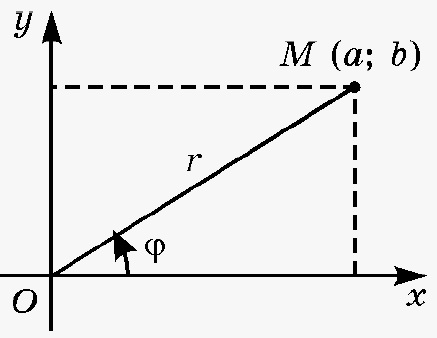
\includegraphics[width=0.4\linewidth]{figures/49_polar_representation_of_complex_number}
	\end{figure*}
	\begin{remark}[Geometrical Interpretation]
		The \textbf{modulus} is the \emph{distance} from the point to the origin.
	\end{remark}
	\begin{remark}[Geometrical Interpretation]
		The \textbf{conjugate} is the \emph{reflection} of the point about the real ($x$) axis.
	\end{remark}
	
	
	\subsection{Polar Coordinates}
	\subsubsection{Coordinate Conversion}
		\par Consider a complex number represented by $(a,b)$ in Cartesian coordinate and $(r, \theta)$ in polar coordinate.
		\begin{figure*}[h]
			\centering
			\begin{tabular}{|c|c|}
				\hline
				Cartesian & Polar \\
				\hline
				$(a, b)$ & $(\sqrt{a^2 + b^2}, \arctan(\frac{b}{a}))$ \\
				\hline
				$(r \cos(\theta), r \sin(\theta))$ & $(r, \theta)$ \\
				\hline
			\end{tabular}
		\end{figure*}
		\begin{remark}
			$\arctan(\frac{b}{a})$ gives multiple solutions due to the periodicity of $\tan$. We need to use the signs of real and imaginary values to determine which value of $\arctan{\frac{b}{a}}$ to take.
		\end{remark}
		
		\begin{example}
			Consider $1+i$, it could be represented as $(1,1)$ in Cartesian coordinate. Converting it into polar coordinates gives $(\sqrt{2}, \frac{\pi}{4})$. Converting back gives
			\begin{gather*}
				1 + i = \sqrt{2}(\cos(\frac{\pi}{4}) + i \sin(\frac{\pi}{4})) \\
				= \sqrt{2} (\cos(\frac{\pi}{4} + 2\pi k) + i \sin(\frac{\pi}{4} + 2 \pi k)),\ \forall k \in \mathbb{Z}
			\end{gather*}
		\end{example}
		
		\subsubsection{Multiplication in Polar Coordinates}
		\par Consider the product of two complex numbers $r_1 (\cos(\theta_1) + i \sin(\theta_1))$ and $r_2 (\cos(\theta_2) + i \sin(\theta_2))$:
		\begin{gather*}
			r_1 (\cos(\theta_1) + i \sin(\theta_1)) \times r_2 (\cos(\theta_2) + i \sin(\theta_2)) \\
			= r_1 r_2 \Big[
				\Big(\cos(\theta_1) \cos(\theta_2)
				 - \sin(\theta_1) \sin(\theta_2) \Big) + 
				 i \Big(
				 	\cos(\theta_1)\sin(\theta_2) + \sin(\theta_1) \cos(\theta_2)
				 \Big)
				\Big] \\
			\tx{By triangle inequality} \\
			= r_1 r_2 \Big ( \cos(\theta_1 + \theta_2) + i \sin(\theta_1 + \theta_2)\Big)
		\end{gather*}
		
		\begin{example}
			Every complex number has a square root. (Generalized idea: \ul{complex field is algebraically closed}.)
			\begin{proof}
				Let $z = r(\cos(\theta) + i \sin(\theta)) \in \mathbb{C}$. \\
				Consider $w = \sqrt{r} (\cos(\frac{\theta}{2}) + i \sin(\frac{\theta}{2}))$ \\
				By above result, we could easily verify that $w^2 = z$. \\
				Notice that, $w = \sqrt{r}\Big(\cos(\frac{\theta}{2} + \pi) + i \sin(\frac{\theta}{2} + \pi) \Big)$ is also a square root of $z$.
			\end{proof}
		\end{example}
	
	\section{Lecture 19 Oct. 22 2018}
		\subsection{De Moivre's Theorem}
		\begin{theorem}(De Moivre's Theorem)
			Let $z = r[\cos(\theta) + i \sin(\theta)] \in \mathbb{C}$, and the $n^{th}$ power of $z$ is given by
			\[
				(r[\cos(\theta) + i \sin(\theta)])^n = r^n [\cos(n\theta) + i \sin(n \theta)],\ \forall n \in \mathbb{N}
			\]
		\end{theorem}
		\begin{proof}
			(By induction) \\
			\textbf{Base Case} for $n=1$, obviously $z^1 = z$ \\
			\textbf{Inductive Step} let $k \in \mathbb{N}$, \\
			suppose $z^k = r^k [\cos(k \theta) + i \sin(k \theta)]$ \\
			Consider $z^{k+1}$, \\
			\begin{gather*}
				r^{k+1} = r^k [\cos(k \theta) + i \sin(k \theta)] \times r[\cos(\theta) + i \sin(\theta)] \\
				= r^{k+1} \Big[
					(\cos(k \theta) \cos(\theta) - \sin (k \theta) \sin(\theta)) + 
					i (\cos(k \theta) \sin(\theta) + \sin(k \theta) \cos(\theta))
				\Big] \\
				\tx{By Triangle Identity} \\
				= r^{k+1} \big[ \cos((k+1)\theta) + i \sin((k+1) \theta) \big ]
			\end{gather*}
			We could then conclude what the theorem stated by principle of mathematical induction.
		\end{proof}
		
		\begin{example}
			Calculate $(1+i)^8$. 
			\begin{proof}[Solution]
				$1+i$ can be written as $(1,1)$ in Cartesian coordinate. \\
				Then it can be converted into Polar coordinate as 
				\[
					\sqrt{2} \Big ( \cos(\frac{\pi}{4}) + i \sin(\frac{\pi}{4})\Big)
				\]
				Then by De Moivre's theorem,
				\begin{gather*}
					\Big( \sqrt{2} \Big ( \cos(\frac{\pi}{4}) + i \sin(\frac{\pi}{4})\Big) \Big)^8 \\
					= (\sqrt{2})^8 \Big ( \cos(\frac{\pi}{4} \times 8) + i \sin(\frac{\pi}{4} \times 8)\Big) \\
					= 16 \times \Big ( \cos(2\pi) + i \sin(2\pi)\Big) \\
					= 16 (\cos(0) + i \sin(0)) \\
					= 16
				\end{gather*}
			\end{proof}
		\paragraph{Geometrically Interpretation}\hl{rotates the vector anti-clockwise by $(n-1)\theta$-radius and enlarge the magnitude by factor of $n$.}
		\end{example}
		
		\subsection{Roots of Unity}
		\begin{example}
			Find all roots of $z^2 = 1$, where $z \in \mathbb{C}$. 
			\begin{proof}[Solution]
				In polar coordinates, let $z = r (\cos \theta + i \sin \theta)$. \\
				Thus by De Moivre's Theorem, $z^2 = r^2 (\cos (2\theta) + i \sin(2\theta))$. \\
				And $1 = 1 (\cos(0+2k\pi) + \sin(0+2k\pi)),\ k \in \mathbb{Z}$ in polar coordinate. \\
				Solving the equation $z^2 = 1$ gives \\
				\[
					\begin{cases}
						r^2 = 1 \\
						2\theta = 2k\pi,\ k \in \mathbb{Z}
					\end{cases}
				\]
				We can conclude that $r=1$ since it represents a \emph{distance} and $r \in \R_{\geq 0}$. \\
				\begin{itemize}
					\item $k=0:\quad r=1,\ \theta = 0 \rightarrow 1(\cos(0) + i \sin(0)) = 1$ 
					\item $k=1:\quad r=1,\ \theta = \pi \rightarrow 1(\cos(\pi) + i \sin(\pi)) = -1$ 
					\item $k=2:\quad r=1,\ \theta = 2\pi \rightarrow 1(\cos(2\pi) + i \sin(2\pi)) = 1$
				\end{itemize}
			\end{proof}
			From the repeating pattern we can conclude that $\forall k \in \mathbb{Z}$ \footnote{The case $k<0$ is covered by symmetry.} \[z = 1 (\cos(\pi k) + i \sin(\pi k)) = \pm 1\]
		\end{example}
		
		\begin{example}
			Find all roots of $z^n = 1$
			\begin{proof}[Solution]
				\begin{gather*}
					z^n = r^n [\cos(n\theta) + i \sin(n \theta)] \\
					1 = 1(\cos(2k\pi) + i \sin(2k\pi)) \\
					\implies r = 1 \\
					\land n\theta = 2 k \pi \iff \theta = k \frac{2\pi}{n} 
				\end{gather*}
				Consider cases 
				\begin{itemize}
					\item $k=0:\quad r=1,\ \theta=0$
					\item $k=1:\quad r=1,\ \theta=\frac{2\pi}{n}$
					\item $k=2:\quad r=1,\ \theta=2\frac{2\pi}{n}$
					\item $k=3:\quad r=1,\ \theta=3\frac{2\pi}{n}$
				\end{itemize}
				Until $k=n$, we have $r=1 \land \theta=n\frac{2\pi}{n}=2\pi$, where $z|_{k=n} = z|_{k=0}$ and the root starts repeating. \\
				There are $n$ roots in total,
				\[
					z = \cos(k \frac{2\pi}{n}) + \sin(k \frac{2\pi}{n}),\ k \in \{0, 1, \dots, n-1\}
				\]
			\end{proof}
		\end{example}
		\begin{example}
			Solve $z^3 = 1$
		\end{example}
		\begin{example}
			Solve $z^4 = 1$
		\end{example}
		\paragraph{Geometrically Interpretation} Divides the unit ball into $n$ equal slices.
		\begin{example}
			Solve $z^3 = 2 + 2 i$
			\begin{proof}[Solution]
				In polar coordinate, 
				\[
					2+2i = \sqrt{8} \Big(\cos(\frac{\pi}{4} + 2k\pi) + i \sin(\frac{\pi}{4} + 2k\pi) \Big)
				\]
				We have to solve 
				\begin{gather*}
					3\theta = \frac{\pi}{4} + 2k\pi,\ k \in \mathbb{Z} \\
					\implies \theta = \frac{\pi}{12} + k \frac{2\pi}{3},\ k \in \mathbb{Z}
				\end{gather*}
				And clearly $r = \sqrt{2}$. And roots are fond by plugging in $k$ with $0,1,2$.
				\[
					\begin{cases}
						z_1 = \sqrt{2} (\cos(\frac{\pi}{12}) + i \sin(\frac{\pi}{12})) \\
						z_2 = \sqrt{2} (\cos(\frac{\pi}{12} + \frac{2\pi}{3}) + i \sin(\frac{\pi}{12} + \frac{2\pi}{3})) \\
						z_3 = \sqrt{2} (\cos(\frac{\pi}{12} + \frac{4\pi}{3}) + i \sin(\frac{\pi}{12} + \frac{4\pi}{3}))
					\end{cases}
				\]
			\end{proof}
		\end{example}
		
	\section{Lecture 20. Oct. 24 2018}
	\begin{theorem}[The Fundamental Theorem of Algebra]
		Every \emph{non-constant} polynomial (with complex coefficients) has a complex root.
		i.e. for 
		\[
			p(z) = a_n z^n + a_{n-1} z^{n-1} + \dots + a_1 z + a_0,\quad a_i \in \mathbb{C},\ n\geq 1
		\]
		there exists $r \in \mathbb{C}$ such that $p(r) = 0$.
	\end{theorem}
	\begin{example}
		Let $p(x) = x^3 -3x^2 - 9x + 27$, $p(x) = (x-3)^2 (x+3)$. \\
		\textbf{Interpretation} \emph{Linear polynomials (polynomials of degree 1) are building blocks of all polynomials.}
	\end{example}
	
	\begin{theorem}[Long Division]
		Suppose $p(z)$ is a non-constant polynomial and $r \in \mathbb{C}$, there exists a polynomial $q(z) \in \mc{P}$ and $c \in \mathbb{C}$ such that
		\[
			p(z) = q(z)(z-r) + c
		\]
		where $c$ is the \emph{reminder} of long division.
	\end{theorem}
	
	\begin{definition}
		A polynomial $f(z)$ is a \textbf{factor} of another polynomial $p(z)$ if 
		\[
			\exists q(z) \in \mc{P},\ s.t.\ p(z) = f(z)q(z)
		\]
	\end{definition}
	
	\begin{theorem}[Factor Theorem]
		A complex number $r$ is a root of a polynomial $p(z)$ if and only if $(z-r)$ is a factor of $p(z)$.
	\end{theorem}
	\begin{proof}
		($\impliedby$) Suppose $(z-r)$ is a factor. \\
		By definition of factor, $\exists q(z) \in \mc{P}$ such that $p(z) = q(z)(z-r)$. \\
		Plugging in $r$ gives $p(r) = q(r)(r-r) = 0$ and suggests $r$ is a root of $p(z)$. \\
		($\implies$) Suppose $r$ is a root of $p(z)$. \\
		By the theorem of long division, $\exists q(z) \in \mc{P}$ and $c \in \mathbb{C}$ satisfying \\
		$p(z) = q(z)(z-r) + c$. \\
		Plugging in $z=r$ gives $p(r) = q(r)(r-r) + c = 0$, which implies $c=0$. \\
		That's $p(z) = q(z)(z-r)$.
	\end{proof}
	
	\begin{theorem}[Extended Fundamental Theorem of Algebra]
		A non-zero\footnote{For zero polynomial, it has infinitely many roots.} polynomial of degree $n$ has exactly $n$ roots, counting multiplicities.
	\end{theorem}
	\begin{proof}
		Let $p(z) \in \mc{P}$ with degree $n \geq 0$ and suppose $p(z)$ is non-zero. \\
		Case 1: $n=0$, then $p(z)$ has 0 roots. \\
		Case 2: $n \geq 1$, by the fundamental theorem of algebra, \\
		$p(z)$ has a root $r_1 \in \mathbb{C}$. \\
		By factor theorem, $\exists q_1(z) \in \mc{P}(\mathbb{C}),\ s.t.\ p(z) = (z-r_1)q_1(z)$. \\
		Note that $q_1(z)$ has degree of $n-1$. \\
		If $n-1 \geq 1$, repeating above argument and we have \\
		$\exists r_2 \in \mathbb{C},\ \exists q_2(z) \in \mc{P}(\mathbb{C}),\ s.t.\ q_1(z) = (z-r_2)q_2(z)$. \\
		Note that $q_2(z)$ has degree of $n-2$. \\
		Equivalently $p(z) = (z-r_1)(z-r_2)q_2(z)$. \\
		Iterating till $q_i(z)$ has degree 0 (i.e. constant), this will be achieved after exactly $n$ iterations. \\
		Aggregately, we can factorize $p(z)$ into 
		\[
			p(z) = (z-r_1)(z-r_2)\dots(z-r_n)q_n
		\]
		where $q_n$ is a constant. \\
		Obviously there are $n$ (possibly repeating) roots, namely $r_1, r_2, \dots, r_n$.
	\end{proof}

	\section{Lecture 21. Oct. 29 2018}
		\begin{lemma}[Triangle Inequality]
			\[
				|z_1 + z_2| \leq |z_1| + |z_2|,\ \forall z_1, z_2 \in \mathbb{C}
			\]
		\end{lemma}

		\begin{lemma}[Extended version of triangle inequality]
			\[
				| \sum_{i=1}^{n} {z_i} | \leq \sum_{i=1}^{n} |z_i|,\ \forall (z_i) \in \mathbb{C}^n
			\]
		\end{lemma}

		\begin{definition}
			A \textbf{closed curve in the plane} is a continuous function mapping from $[0, 2\pi]$ to $\mathbb{C}$ such that its values at $0$ and $2\pi$ are the same.
		\end{definition}

		\begin{definition}
			If $\phi(t): [0, 2\pi] \to \mathbb{C}$ is a closed curve that \hl{does not go through the origin}, its \textbf{winding number} is the number of times a vector from the origin to a point on the curve winds around the origin as $t$ goes from $0$ to $2\pi$.
		\end{definition}

		\begin{example}
			Consider 
			\[
				\phi(t) = f(t) + i(g)
			\]
			where $f,g: [0, 2\pi] \to \R$ are continuous. Then $\phi(t)$ is continuous.
		\end{example}

		\begin{example}
			Consider 
			\[
				\phi(t) = \cos(t) + i\sin(t)
			\]
			the function above is a closed curve with winding nunber $+1$.
		\end{example}

		\begin{remark}
			If points on the curve go around the origin \emph{anti-clockwise} as $t$ goes from $0$ to $2\pi$, then we consider the winding number to be \emph{negative}.
		\end{remark}

		\begin{example}
			Curve $\phi(t) = \cos(3t) + i \sin(3t)$ has winding number $+3$.
		\end{example}

		\begin{example}
			Curve $\phi(t) = 27\cos(4t) + 27 i \sin(4t)$ has winding number $+4$.
		\end{example}
		
		\begin{example}
			Curve $\phi(t) = \sin(t) + i \cos(t)$ has winding number $-1$.
		\end{example}
		
		\begin{example}
			A non-zero constant (e.g. $\phi(t)=3+4i$) is closed and not passing the origin, it has winding number $0$.
		\end{example}
		
		\begin{remark}
			\hl{The notation of winding number only apply to closed curves that do \textbf{not} passes the origin.}
		\end{remark}
		\subsection{Proof of the Fundamental Theorem of Algebra}
		\begin{proof}
			Idea: prove by contradiction. \\
			Suppose $p(z)$ is a non-constant polynomial with no roots. \\
			i.e. 
			\[
				p(z) \neq 0,\ \forall z \in \mathbb{C}
			\]
			and degree of $p(z) = n > 0$. \\
			For each radius $R>0$ define 
			\[
				\phi_R(t) := R(\cos(t) + i \sin(t))
			\]
			Then for each $R>0$, let 
			\[
				p_R(t) := p(\phi_R(t))
			\]
			note that $p_R(t): [0, 2\pi] \to \mathbb{C}$ and it's a closed curve. \\
			Also note that since $p_R(t) \neq 0\ \forall t \in [0, 2\pi]$, $p_R(t)$ does not go through the origin. \\
			We will show that
			\begin{enumerate}
				\item If $R$ is large enough then the winding number of $p_R(t) = deg(p(z))$.
				\item If $R$ is small enough then the winding number of $p_R(t) = 0$.
			\end{enumerate}
			But the winding number of $p_R(t)$ is a continuous function of $R$ and it has co-domain of integers. Then it must be the case that $p_R(t)$ is constant, but this contradicts our assumption that $deg(p(z)) > 0$.
		\end{proof}
		
	\section{Lecture 22. Oct. 31 2018}
		\paragraph{Recall} the outline of proving the Fundamental Theorem of Algebra. 
		\newline
		Suppose $p(z)$ is a non-=constant polynomial with no roots. i.e.
		\[
			p(z) \neq 0\quad \forall z \in \mathbb{C}
		\]
		Let 
		\[
			p_R(t) := p(\phi_R(t))
		\]
		where $\phi(t): [0, 2\pi] \to \mathbb{C} = R(\cos(t) + i\sin(t))$.
		\newline
		And we well show
		\begin{enumerate}
			\item $R$ is large $\implies$ winding number of $p_R(t) = degree(p(z))$
			\item $R$ is small $\implies$ winding number of $p_R(t) = 0$.
		\end{enumerate}
		\begin{proof}
			Let $q(z) = z^n$, where $n$ is the degree of polynomial $p(z)$. \\
			Let $L_R(t) = q(\phi_R(t))$. \\
			Note that
			\begin{gather*}
				L_R(t) = q(\phi_R(t)) \\
				= q(R(\cos(t) + i\sin(t))) \\
				= R^n (\cos(nt) + i\sin(nt))
			\end{gather*}
			so $L_R(t)$ has winding number $n$. \\
			\begin{lemma}
				Let $L(t)$ and $M(t)$ be 2 closed curves not passing through the origin. \\
				Suppose 
				\[
					| L(t) - M(t) | < | L(t) |\quad \forall t \in [0, 2\pi]
				\]
				then $L(t)$ and $M(t)$ have the same winding number.
			\end{lemma}
			\emph{We are \textbf{not} going to prove this lemma}. \\
			\begin{proof}[Proof. Proposition 1]
				Since $L_R(t) = \phi_R(t)^n$, \\
				Suppose 
				\[
					p(\phi_R(t)) = a_n z^n + a_{n-1} z^{z-1} + \dots + a_1 z + a_0
				\]
				WLOG, assume $a_n=1$. \\
				Then 
				\[
					p_R(t) = \phi_R(t)^n + a_{n-1} \phi_R(t)^{n-1} + \dots + a_1 \phi_R(t) + a_0
				\]
				and 
				\begin{gather*}
					|L_R(t) - p_R(t)| = |a_{n-1} \phi_R(t)^{n-1} + \dots + a_1 \phi_R(t) + a_0| \\
					\leq |a_{n-1}\phi_R(t)^{n-1}| + \dots + |a_0| \\
					= |a_{n-1}| |\phi_R(t)|^{n-1} + |a_{n-2}| |\phi_R(t)|^{n-2} + \dots + |a_1| |\phi_R(t)| + |a_0| \\
					= |a_{n-1}| R^{n-1} + |a_{n-2}| R^{n-2} + \dots + |a_1| R + |a_0| \\
					\tx{Choosing } R > \max \{1, \sum_{i=1}^{n-1}|a_i|\} \\
					< |a_{n-1}| R^{n-1} + |a_{n-2}| R^{n-1} + \dots + |a_1| R^{n-1} + |a_0| R^{n-1} \\
					= R^{n-1} \sum_{i=1}^{n-1} |a_i| \\
					< R^n = |L_R(t)|
				\end{gather*}
				Thus we have shown that
				\[
					|L_R(t) - p_R(t)| < |L_R(t)|,\quad \forall t \in [0, 2\pi]
				\]
				by choosing $R$ large enough. By previous lemma, we conclude that $p_R(t)$ has the same winding number as $L_R(t)$, which is $n$. \\
			\end{proof}
			\begin{proof}[Proof. Proposition 2]
				Note $p(0) = a_0 \neq 0$ since we assumed $p$ has no roots. \\
				Since $p(z)$ is a polynomial so its continuous. (of course near $0$) \\
				\[
					\forall \epsilon > 0,\ \exists \delta > 0\ s.t.\ 0 < |z - 0| < \delta \implies |p(z) - p(0)| < \epsilon 
				\]
				Since $p(0) \neq 0$ and the quadrant(excluding axes) containing $a_0$ is open.\\
				There exists $\epsilon$ such that all points $z$ in $\mc{B}(\epsilon, a_0)$ are in that quadrant. \\
				There exists $\delta > 0$ satisfying the continuity definition above and we choose 
				\[
					R = \frac{\delta}{2}
				\]
				Then all $z$ in set $\{\phi_R(t):t\in [0, 2\pi]\}$ are mapped into $\mc{\epsilon, a_0}$, and of course in the quadrant containing $a_0$.\\
				Therefore the winding number of $p_R(t)$ is 0.
			\end{proof}
			altogether with the fact that winding number of $p_R(t)$ is a continuous function from $R_{>0}$ to integers, we conclude that $p_R(t)$ is constant. \\
			This conclusion contradicts our assumption that $p(z)$ is non-constant, i.e. $n \neq 0$. \\
			Thus $p(z)$ has root.
		\end{proof}
		
	\section{Lecture 23. Nov. 2 2018}
		\begin{proposition}
			The winding number transformation of $p_R(t) = p(\phi_R(t))$, $W: \R_{> 0} \to \mathbb{Z}$ is continuous in $R$.
		\end{proposition}
		\begin{proof}
			For small enough $\epsilon > 0$, \\
			Consider 
			\begin{equation}
				|p_{R + \epsilon}(t) - p_R(t)| < |p_R(t)|,\ \forall t
			\end{equation}
			we will show (1) is true for sufficiently small $\epsilon > 0$. \\
			By lemma 22.1, $p_{R+\epsilon}(t)$ and $p_R(t)$ have the same winding number. \\
			Let 
			\begin{equation}
				p(z) = z^n + a_{n-1}z^{n-1} + \dots + a_1 z + a_0
			\end{equation}
			Then 
			\begin{gather}
				\big| p_{R+\epsilon}(t) - p_R(t) \big| = \big| (\phi_{r+\epsilon}(t)^n + a_{n-1}\phi_{r+\epsilon}(t)^{n-1} + \dots) - (\phi_{R}(t)^n + \dots) \big| \\
				= \big| (\phi_{r+\epsilon}(t)^n - \phi_R(t)^n) + a_{n-1}(\phi_{r+\epsilon}(t)^{n-1} - \phi_R(t)^{n-1}) + \dots \big| \\
				= \big| [(R+\epsilon)^n - R^n] e^{int} + a_{n-1} [(R+\epsilon)^{n-1} - R^{n-1}] e^{i(n-1)t} + \dots \big| \\
				\leq \big| (R+\epsilon)^n - R^n \big | \big |e^{int} \big| + \big| a_{n-1} \big| \big | (R+\epsilon)^{n-1} - R^{n-1} \big | \big | e^{i(n-1)t} \big | + \dots + \big |a_1 \big| \big |e^{it} \big |
			\end{gather}
			note that
			\begin{equation}
				\abs{e^{ijt}} = 1,\quad \forall j \in \{1, 2, \dots, n\}
			\end{equation}
			Thus
			\begin{gather}
				\abs{p_{R+\epsilon}(t) - p_R(t)} \leq \sum_{j=1}^n \abs{(R + \epsilon)^j - R^j}
			\end{gather}
			Note that we can make $\abs{(R+\epsilon)^k - R^k}$ as small as we want by specifying a sufficiently small $\epsilon$ since $x^k$ is continuous. \\
		\end{proof}
		
		\begin{definition}
			A set $S$ is \textbf{finite} if there exists some $n\in \mathbb{N}$ such that the elements of $S$ can be paired with the elements in set $\{1, 2, \dots, \textcolor{red}{n}\}$. Equivalently, we can label the elements of $S$ as $s_1, s_2, \dots s_n$.
		\end{definition}
		
		\begin{definition}
			A set is \textbf{infinite} if it is not finite.
		\end{definition}
		
		\begin{definition}
			Two sets $S$ and $T$ \footnote{$S$ and $T$ are \textbf{not} necessarily finite.} have the same \textbf{cardinality} if and only if there exists a \emph{bijection} between them. Written as $\abs{S} = \abs{T}$.
		\end{definition}
		
	\section{Lecture 24. Nov 12. 2018}
		\begin{example}[Infinite Sets with Same Cardinality]
			Let $S = \mathbb{N}$ and $T = \{2,4,6,\dots\}$, easy to construct a bijective mapping $f:S\to T$ defined as $f(n) = 2n$ to show $S$ and $T$ have the same cardinality.
		\end{example}

		\begin{example}[Infinite Sets with Same Cardinality]
			Let $S = \mathbb{N}$ and $T = \{2,3,4,\dots\}$, easy to construct a bijective mapping $f:S\to T$ defined as $f(n) = n+1$ to show $S$ and $T$ have the same cardinality.
		\end{example}
		
		\begin{remark}[How to prove a set has the same cardinality as natural numbers]
			If $\abs{\mathbb{N}} = \abs{T}$, then $\exists$ bijection $f:\mathbb{N} \to T$. That's we can \emph{enumerate} elements in $T$ with $f(n)$: 
			\[
				t_1 = f(1),\ t_2 = f(2),\dots \quad \forall t_i \in T
			\]
		\end{remark}
		
		\begin{definition}
			Let $T$ be a set, if $\abs{T} = \abs{\mathbb{N}}$, then $T$ is \textbf{countably infinite} and written as $\abs{T} = \aleph_0$.
		\end{definition}
		
		\begin{definition}
			A set is \textbf{countable} if it is either finite or countably infinite.
		\end{definition}
		
		\begin{theorem}
			Set $S = \mathbb{Q}^+$ is countable infinite.
		\end{theorem}
		\begin{proof}
			\begin{figure*}[h]
				\centering
				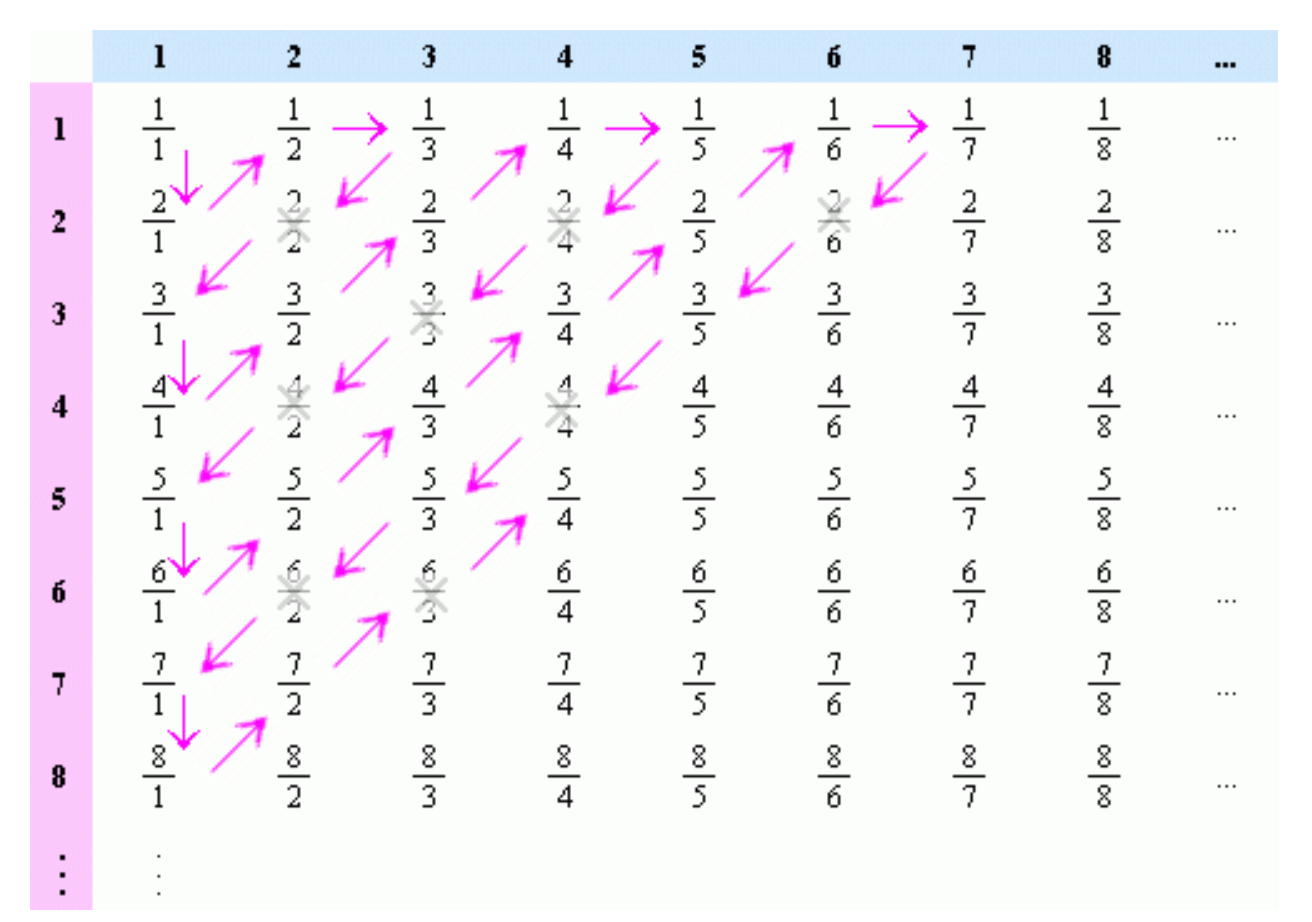
\includegraphics[width=0.5\linewidth]{figures/countinfproof}
			\end{figure*}
		\end{proof}
		\begin{proof}(alternative.)
			Note that the Cartesian product of countably infinite sets is countably infinite. \\
			Then, for all $\frac{p}{q} \in \mathbb{Q}^+$, where $p, q \in \mathbb{N}$ and $p, q$ are relatively prime. \\
			Setup bijection $\phi:\mathbb{Q}^+ \to \mathbb{N}^2$, defined as $\phi(\frac{p}{q}) = (p,q)$. \\
			So $\abs{\mathbb{Q}^+} = \abs{\mathbb{N}^2}$. \\
			Thus $\mathbb{Q}^+$ is countably infinite.
		\end{proof}
		
		\begin{theorem}
			Let $[0,1]$ be the set of all real numbers between 0 and 1. $[0,1]$ is not infinitely countable.
		\end{theorem}
		\begin{proof}
			(Prove by contradiction) \\
			Suppose we can list all real numbers between 0 and 1 as 
			\begin{gather*}
				a_1 = 0.a_{11}a_{12}a_{13}\dots \\
				a_2 = 0.a_{21}a_{22}a_{23}\dots \\
				a_3 = 0.a_{31}a_{32}a_{33}\dots \\
				\vdots
			\end{gather*}
			Consider another real number in $[0,1]$ constructed as following
			\[
				x = 0.x_1 x_2 x_3 \dots \tx{ where } x_i = \begin{cases}
					6 \tx{ if } a_{ii} = 5 \\
					5 \tx{ otherwise}
				\end{cases}
			\]
			Note that the first decimal of $x$($x_1$) is not the same as the first decimal of $a_1$($a_{11}$), so $x \neq a_1$. \\
			Similarly, the second decimal of $x$($x_2$) is not the same as the second decimal of $a_2$($a_{22}$), so $x \neq a_2$, \\
			It is easy to show that $x \neq a_i,\ \forall i$. So $x$ is a real number between 0 and 1 not included in the table above. \\
			Contradicting the assumption that we could list all real numbers between 0 and 1 in a table. \\
			Thus $[0,1]$ is not infinitely countable.
		\end{proof}
		
	\section{Lecture 25. Nov. 14 2018}
		\begin{notation}[the Cardinality of continuum]
			$\abs{[0,1]}=C$
		\end{notation}
		
		\begin{definition}
			$|S| \leq |T|$ if there exists a subset $T_0 \subseteq T$ such that $|T_0| = |S|$. Or, equivalently, there exists an injection maps from $S$ to $T$.
		\end{definition}
		
		\begin{definition}
			$|S| < |T|$ if $|S| \leq |T|$ and $|S| \neq |T|$.
		\end{definition}
		
		\begin{proposition}
			$|\mathbb{N}| < |[0, 1]|$ (i.e. $\aleph_0 < C$)
			\begin{proof}
				We've already shown that $|\mathbb{N}| \neq |[0,1]|$. \\
				Consider injection $f:\mathbb{N}\to [0,1]$ defined as $f(n) = \frac{1}{n}$. \\
				Therefore $|\mathbb{N}| \leq |[0,1]|$. \\
				Or equivalently the subset of $[0,1]$ defined as $\{\frac{1}{n}:n \in \mathbb{N}\}$ has the same cardinality as $\mathbb{N}$. \\
				Thus, by definition, $|\mathbb{N}| < |[0, 1]|$.
			\end{proof}
		\end{proposition}
		
		\begin{theorem}[Schödre-Bernstein-Cantor Theorem]
			Let $S$ and $T$ be two sets then
			\[
				|S| \leq |T| \land |S| \geq |T| \implies |S| = |T|
			\]
			\begin{proof}
				
			\end{proof}
		\end{theorem}
		
		\begin{proposition}
			Let $a,b,c,d \in \R$ satisfying $a<b$ and $c<d$, then
			\[
				|[a,b]| = |[c,d]| = C
			\]
			\emph{Every closed interval has the same cardinality}.
			\begin{proof}
				Consider mapping $f(x) = (d-c)\frac{x-a}{b-a}+c$. \\
				Obviously, $f:[a,b] \to [c, d]$ and bijective. \\
				And therefore it's inverse is a bijection from $[c,d]$ to $[a,b]$. \\
				Thus those two closed intervals have the same cardinality.
			\end{proof}
		\end{proposition}
		
		\begin{proposition}
			$|\R| = |(-\frac{\pi}{2}, \frac{\pi}{2})|$.
			\begin{proof}
				Consider bijection $f(x):= \tan(x)$.
			\end{proof}
		\end{proposition}
		
		\begin{proposition}
			$|[0, 1]| = |(0, 1)|$.
			\begin{proof}
				Step 1. Consider bijection $f(x):=x$ and obviously $|(0, 1)| \leq |[0, 1]|$. \\
				Step 2. As shown before, all closed interval have the same cardinality. Thus $|[0, 1]| = |[\frac{1}{4}, \frac{1}{2}]|$. And clearly $[\frac{1}{4}, \frac{1}{2}] \subsetneq (0, 1)$. \\
				So $|[0,1]| = |[\frac{1}{4}, \frac{1}{2}]| \leq |(0, 1)|$. \\
				By Schödre-Bernstein-Cantor theorem, $|[0,1]|=|(0,1)|$
			\end{proof}
		\end{proposition}
		
		\begin{proposition}
			Above result can be generalized to arbitrary open and closed intervals, i.e.
			\[
				|[a,b]| = |(c,d)|
			\]
		\end{proposition}
	\section{Lecture 26 Nov. 16 2018}
		\begin{theorem}[A Countable Union of Countable Sets is Countable]
			If $|S_i| = \aleph_0,\ \forall i \in \mc{I}$ where $|\mc{I}| = \aleph_0$, then
			\[
				|\cup_{i\in\mc{I}}S_i| = \aleph_0
			\]
		\end{theorem}
		\begin{proof}
			The proof involving finite union or all finite sets is trivial, here we consider countable as infinitely countable.\\
			Since $S_1 \subseteq \cup_{i\in\mc{I}}S_i \implies |S_1| \leq |\cup_{i\in\mc{I}}S_i| \implies |\cup_{i\in\mc{I}}S_i| \geq \aleph_0$. \\
			Then use the snake argument (count along the diagonal) we can easily prove that the set $\cup_{i\in\mc{I}}S_i$ is countable.
		\end{proof}
		\begin{example}
			$|\mathbb{Q}|=\aleph_0$.
			\begin{proof}
				Obviously, $\mathbb{Q} = \mathbb{Q}^- \cup \{0\} \cup \mathbb{Q}^+$. \\
				Also we've shown that $|\mathbb{Q}^+| = \aleph_0$. \\
				A bijection can be set up between $\mathbb{Q}^+$ and $\mathbb{Q}^-$. \\
				And $\{0\}$ is finite. \\
				So $\mathbb{Q}$ is a finite (countable) union of three countable sets. \\
				Therefore $|\mathbb{Q}| = \aleph_0$.
			\end{proof}
		\end{example}
		
		\begin{example}
			$|\mathbb{N}^2| = \aleph_0$ 
			\begin{proof}
				Note that $\mathbb{N}^2 = \cup_{i\in \N}\{(i,j):j\in \N\}$, which is a countable union of countable sets. \\
				So $\N^2$ is countable.
			\end{proof}
		\end{example}
		
		\begin{corollary}
			As a generalization of above example, the Cartesian product of countable sets is countable.
		\end{corollary}
		
		\begin{theorem}
			A countable union of sets with cardinality $c$ also have cardinality $c$.
			\[
				|S_i| = c, \ \forall i = 1,2,3\dots \implies |\cup_{i=1}^\infty S_i| = c
			\]
			\begin{proof}
				$S_1 \subseteq \cup_{i=1}^\infty S_i \implies c = |S_1| \leq \cup_{i=1}^\infty S_i$. \\
				WLOG, assume all sets $S_i$ are disjoint. \\
				(Otherwise, we could construct a new collection of disjoint sets by defining $S_1' = S_1$ and $S_j' = S_j \backslash \cup_{i=1}^{j-1} S_{i}$) \\
				Since $|S_i| = c$, $|S_i| = |(i, i+1)|$. \\
				Therefore, for every $S_i$, there's a bijection between it and open interval $(i, i+1)$. \\
				Easy to shown that there exists a bijection between $\cup_{i=1}^\infty S_i$ and $\cup_{i=1}^\infty (i, i+1) \subseteq \R$. \\
				So, $|\cup_{i=1}^\infty S_i| = |\cup_{i=1}^\infty (i, i+1)| \leq |\R| = c$. \\
				Thus $|\cup_{i=1}^\infty (i, i+1)| \leq c$. \\
				By SBC, $|\cup_{i=1}^\infty (i, i+1)| = c$. \\
			\end{proof}
		\end{theorem}
		
		\begin{example}
			Consider the unit square $S=[0,1]\times [0,1]$. $S$ is an uncountably infinite union of uncountably infinite sets.\\
			Claim $|S| = c$. \\
			\begin{proof}
				$S = \cup_{x\in [0,1]}\{(x,y):y\in[0,1]\}$. \\
				Consider $\{(x, 0):x \in [0,1]\} \subseteq S$, which has cardinality $c$. \\
				Therefore $|S| \geq c$. \\
				Consider the function $f: S \to \{(x, 0):x \in [0,1]\}$ \\
				Consider $(x,y) \in S$ with $x = 0.x_1 x_2 x_3 \dots,\ y=0.y_1 y_2 y_3 \dots$. \\
				Defined $f$ as $f(x, y) = (0.x_1 y_1 x_2 y_2 x_3 y_3\dots, 0)$.\\
				$f$ is injective, therefore $|S| \leq c$. \\
				Thus by SBC, $|S| = c$.
			\end{proof}
		\end{example}
	
	\begin{corollary}
		\[
			|\R^n| = c
		\]
	\end{corollary}
	
	\section{Lecture 27. Nov. 19 2018}
		\begin{theorem}
			Let $S$ be the power set of real numbers, $\mc{P}(\R)$, then $|S| > c$. \footnote{The \textbf{power set} of a set $S$ is defined as the collection of all subsets of set $S$, including $S$ itself and $\emptyset$.}
			\begin{proof}
				\textbf{Part 1} Consider an injection $f: R \to S$ defined as $f(x) = \{x\}$. \\
				Clearly $f$ is injective but not surjective. \\
				Therefore $c = |\R| \leq S$. \\
				\textbf{Part 2} we are going to show $|S| \neq |\R|$ by contradiction. \\
				Suppose $|S| = |\R|$, then there must exists a bijection $g: \R \to S$. \\
				Define the set 
				\[
					\textcolor{red}{T := \{x \in \R: x \notin g(x)\} \subseteq S}
				\]
				We claim that $g$ cannot be surjective by showing that $T \notin g(\R)$. \\
				($g(\R)$ is the image of $g$ on $\R$.) \\
				Suppose $g$ is surjective, then $\exists z \in \R$ s.t. $g(z) = T$. \\
				\emph{Case 1:} $z \in g(z) \implies z \notin T \implies z \notin g(z)$. \\
				\emph{Case 2:} $z \notin g(z) \implies z \in T \implies z \in g(z)$. \\
				Therefore such $z$ cannot exist. \\
				Thus $g$ is not surjective or bijective. \\
				So we cannot construct any bijective transformation between $\R$ and $S$, \\
				Consequently, $|\R| \neq |S|$.
			\end{proof}
		\end{theorem}
		\begin{notation}
			For cardinality of $\mc{P}(\R)$ is denoted as $2^c$.
		\end{notation}
		
		\begin{remark}
			Note that $\aleph_0 < c < 2^c$.
		\end{remark}
		
		\begin{theorem}[10.3.27]
			For every set $S$, $|S| < |\mc{P}(S)|$.
			\begin{proof}
				Proof is similar to the proof above, the key is to consider set
				\[
					T = \{x \in S: x \notin g(x)\} \in \mc{P}(S)
				\]
				and setup contradiction.
			\end{proof}
		\end{theorem}
		
		\begin{corollary}
			There is no largest cardinality.
		\end{corollary}
		
		\begin{definition}[10.3.14]
			Let $\mc{S}$ and $\mc{T}$ be any sets. We will say that $\mc{T}$ \textbf{can be labelled} by set $\mc{S}$ is there is a way of assigning a \hl{finite} sequence of elements of $\mc{S}$ to each element of $\mc{T}$ so that each finite sequence corresponds to at most one element of $\mc{T}$. (i.e. injective assigning)
		\end{definition}
		
		\begin{theorem}[Enumeration Principle]
			The set of \ul{finite} sequences of (elements from) a \ul{countable} set is countable.
		\end{theorem}
		
		\begin{theorem}[Enumeration Principle]
			Every set that can be labelled by a countable set is countable.
		\end{theorem}
		
		\begin{example}
			The set of all finite sequence of $\N$ is countable.
			\begin{proof}
				The set can be expressed as 
				\[
					\cup_{i=0}^{\infty} \{\tx{sequence of } \N \tx{ with length = }i\} = \cup_{i=0}^\infty \N^i
				\]
				\textbf{Note} that we regard $\N^0 = \emptyset$ \\
				which is a (infinitely) countable union of countable sets, and consequently countable. 
			\end{proof}
		\end{example}
		
		\begin{example}
			$\Q^+$ is countable.
			\begin{proof}
				Express positive rationals as 
				\[
					\Q^+ = \{\frac{m}{n}:m, n \in \N, m, n \tx{ are relatively prime.}\}
				\]
				Setup injection $f: \Q^+ \to \N^2$ defined as $f(\frac{m}{n}) = (m,n)$. \\
				Since $\N^2$ can be considered as a set of tuples(finite sequences of length 2) from $\N$,\\
				i.e. $\Q^+$ can be labelled using finite sequences from countable set $\N$. \\
				By enumeration principle, $\Q^+$ is countable, i.e. $|\Q^+| \leq \aleph_0$. 
			\end{proof}
		\end{example}
		
	\section{Lecture 28 Nov. 21 2018}
		\begin{example}
			We've already shown that $|[0,1]| = |(0,1]|$ by
			\begin{gather*}
				(0,1] \subseteq [0,1] \implies |(0,1])| \leq |[0,1]| \\
				|[0,1]| = |[\frac{1}{2}, 1]| \land [\frac{1}{2}, 1] \subseteq (0, 1] \implies |[0, 1]| \leq |(0, 1]| \\
				\implies |[0, 1]| = |(0,1]|
			\end{gather*}
			Now construct a bijection between $[0, 1]$ and $(0, 1]$.\\
			\begin{equation}
				f(x) = \begin{cases}
					1 &\tx{ if } x = 0 \\
					\frac{1}{n+1} &\tx{ if } \exists n \in \N,\ s.t.\ x = \frac{1}{n} \\
					x &\tx{ otherwise}
				\end{cases}
			\end{equation}
		\end{example}
		
		\begin{lemma}
			If $S$ is a infinite set, then $S$ contains a countably infinite That's,
			\[|S| \geq \aleph_0\]
			for all infinite set $S$. And $\aleph_0$ is the \ul{smallest} infinite cardinality.
		\end{lemma}
		\begin{proof}
			Let $SS$ be infinite, \\
			Pick $s_1 \in S$ and $S \backslash \{s_1\}$ is still infinite. \\
			Pick $s_2 \in S\backslash\{s_1\}$ and $S \backslash \{s_1, s_2\}$ is still infinite. \\
			$\vdots$ \\
			Pick $s_k \in S \backslash \cup_{i=1}^{k-1}\{s_i\}$ and $S \backslash \cup_{i=1}^{k}\{s_i\}$ is still infinite. \\
			We've constructed an infinite (countable) list $\{s_1, s_2, \dots\} \subset S$. \\
			Note that, by construction, there's no repeated elements in the constructed list. 
		\end{proof}
		
		\begin{theorem}
			Suppose $S$ is an uncountable (infinite) set and $S_0 \subseteq S$ is a countably infinite subset of $S$, then
			\[
				|S \backslash S_0| = |S|
			\]
		\end{theorem}
		\begin{proof}
			If $S\backslash S_0$ is finite or countable, then $(S\backslash S_1) \cup S_0 = S$ is also countable as a countable union of countable sets, which contradicts our assumption that $S$ is uncountable. So $S \backslash S_0$ is uncountably infinite. \\
			By lemma above, we know there exists a countably infinite set $S_1 \subseteq S \backslash S_0$. \\
			The union $S_0 \cup S_1$ is countably infinite, that's,
			\[
				|S_0 \cup S_1| = |S_1| = \aleph_0
			\]
			So there exists a bijection $g:S_0 \cup S_1 \to S_1$. \\
			Define function $f: S \to S \backslash S_0$ as 
			\[
				f(x) = \begin{cases}
					g(x) &\tx{ if } x \in S_0 \cup S_1 \\
					x &\tx{ otherwise}
				\end{cases}
			\]
			Note that in the first case, bijection $g(S) = S_1$ and in the second case bijection $y(x)=x$ has range $S \backslash S_1$. \\
			Therefore the domains and ranges of the two pieces in piece-wise function $f(x)$ are all disjoint. \\
			So $f(x)$ is bijective, therefore $|S \backslash S_0| = |S|$.
		\end{proof}
	\section{Lecture 29 Nov. 23 2018}
		\begin{theorem}
			A set $S$ is infinite \ul{if and only if} it has a proper subset with same cardinality as $S$.
		\end{theorem}
		\begin{proof}
			($\implies$) \\
			Suppose $S$ is infinite, it has a countable subset $S_0 = \{s_1, s_2, \dots\}$.\\
			Note that $S = (S\backslash S_0) \cup S_0$. \\
			Let $T := S \backslash \{s_1\} \subsetneq S$. \\
			Consider function $f:T \to S$
			\[
				f(x) = \begin{cases}
					s_{i+1} &\tx{ if } x \in S_0 \\
					x &\tx{ if } x \in S \backslash S_0
				\end{cases}
			\]
			Note that $f$ is a piece-wise function and $f(S_0) \cap f(S\backslash S_0) = \emptyset$. \\
			($\impliedby$) \\
			If $S$ is finite, then any proper subset $T$ would have $|T| < |S|$. \\
			The converse part can be shown by showing its contraposition.
		\end{proof}
		
		\begin{theorem}
			The set of all subset of $\N$, $\mc{P}(\N)$, has cardinality $c$.
			\[
				2^{\aleph_0} = c
			\] 
		\end{theorem}
		
		\begin{definition}
			Let $S$ be a set and the \textbf{characteristic function} of set $S_0 \subseteq S$ is a function $f: S \to \{0,1\}$ defined as 
			\[
				f_S(n) = \begin{cases}
					1 &\tx{ if } n \in S_0 \\
					0 &\tx{ if } n \notin S_0
				\end{cases}
			\]
		\end{definition}
		
		\begin{proof}[proof. of above theorem]
			Obviously, we can construct a characteristic function $f_S$ for any set $S \subseteq \N$ and such a constructor is bijective. \\
			There exists a bijection $\phi: \mc{P}(\N) \to \{char.\ func.\} = T$. \\
			Therefore $|\mc{P}(\N)| = |\{char.\ func.\}| = |T|$ \\
			We are going to show $|\mc{P}(\N)| = c$ by showing $|T| = c$. \\
			Define $\varphi: T \to \R$ as $\varphi(f) := 0.f(1)f(2)f(3)\dots$, \\
			$\varphi$ is obviously injective.\\
			Therefore $|T| \leq |\R| = c$. \\
			\newline 
			Consider function $\psi: [0, 1]\to T$ defined in the following way, \\
			for any $x \in [0,1]$, the binary representation of $x$ is 
			\[
				x = \sum_{i=0}^{\infty} b_i 2^{-i} = (b_0 b_1 b_2 b_3 \dots )_2
			\]
			Defined the image $\psi(x)$ as $f$ such that \\
			$f(i) := $ the $i^{th}$ element in the binary representation of $x$. \\
			Consider $x_1, x_2 \in [0,1]$, suppose $\psi(x_1) = \psi(x_2)$, then $x_1$ and $x_2$ have identical binary representation. \\
			Since conversion between binary and decimal representations is bijective, we conclude that $\psi(x_1) = \psi(x_2) \implies x_1 = x_2$. \\
			So that $\psi:[0,1]\to T$ is injective, and $|T| \geq |[0,1]| = c$. \\
			By SBC, we conclude $|T| = c$. \\
			Consequently, $\mc{P}(\N) = c$.
		\end{proof}
		
		\begin{definition}
			A real number is \textbf{algebraic} if there exists a non-zero polynomial with \ul{integer coefficients} that has this number as a root. The set of all algebraic numbers is denoted as $\mc{A}$.
		\end{definition}
		
		\begin{theorem}
			Any \ul{rational} number is algebraic. i.e. 
			\[
				\Q \subseteq \mc{A}
			\]
		\end{theorem}
		\begin{proof}
			Let $\frac{m}{n} \in \Q$, where $m, n \in \Z$.
			Obviously it's a root of polynomial $nx - m$.
		\end{proof}
		
		\begin{theorem}
			\[
				|\mc{A}| = \aleph_0
			\]
			Therefore 
			\[
				\mc{A} \subsetneq \R
			\]
		\end{theorem}
		
		\begin{definition}
			Real numbers that are not algebraic are called \textbf{transcendental}, can be denoted as $\R \backslash \mc{A}$.
		\end{definition}
		
		\begin{example}
			$\pi$ and $e$ are transcendental numbers.
		\end{example}
	\section{Lecture 30. Nov 26 2018}
		\begin{theorem}
			\[
				|\mc{A}| = \aleph_0
			\]
		\end{theorem}
		\begin{proof}
			\textbf{General idea}: we can label each $a \in \mc{A}$ using a finite sequence of integers capturing the coefficients of polynomial having $a$ as a root, altogether with a natural number representing the position order of $a$ as a root. Then $\mc{A}$ can be labelled using countable sets then it's countable.\\
			Note that $\mc{A}$ can be written as
			\[
				\mc{A} = \cup_{i \in \N} \mc{A}_i
			\]
			where $\mc{A}_i$ denotes the set of $x \in \R$ where $x$ is a root of a polynomial with integer coefficients and degree $i$. \\
			Note that for any polynomial of degree $n$
			\[
				a_0 + a_1 x + a_2 x^2 + \cdots + a_n x^n
			\]
			can be written as a $(n + 1)$-tuple:
			\[
				(a_n, a_{n-1}, a_{n-2}, \dots, a_1, a_0) \in \Z^{n+1}
			\]
			By the fundamental theorem of algebra, a polynomial of degree $i$ has $i$ roots, including the multiplicities and complex roots. \\
			For each polynomial of degree $i$, list its roots in some order and append the index of each root $j \in \{1,2,\dots,i\}$ to the $(i+1)$-tuple representing the polynomial. \\
			So that 
			\[
				(a_n, \dots, a_1, a_0, j) \in \Z^{i+1}\times \{1,2,\dots,i\}
			\]
			provides an unique label (i.e. a bijection) to locate every root of every polynomial with integer coefficients and degree $i$. \\
			i.e.
			\begin{gather*}
				|\{\tx{all roots, including complex and duplicates, of polynomials of degree $i$}\}| \\
				= |\Z^{i+1}\times \{1,2,\dots,i\}|
			\end{gather*}
			And note that algebraic numbers are all real, so we have to exclude those complex roots from our locator system. \\
			Also, we have to drop the duplicate roots from above label system. \\
			Since $\Z$ and $\{1,2,\dots,i\}$ are countable,
			\[
				|\Z^{i+1}\times \{1,2,\dots,i\}| = \aleph_0
			\]
			So that 
			\[
				|\mc{A}_i| \leq |\Z^{i+1}\times \{1,2,\dots,i\}| = \aleph_0
			\]
			Lastly, since we've shown that all rational numbers are algebraic and the set of rational numbers is countable. 
			\[
				\aleph_0 = |\Q| \leq |\mc{A}|
			\]
			Consequently,
			\[
				|\mc{A}_i| = \aleph_0,\ \forall i \in \N
			\]
			and $\mc{A}$ is a countable union of countable $\mc{A}_i$, so 
			\[
				|\mc{A}| = \aleph_0
			\]
		\end{proof}
		
		\begin{notation}
			$\R \backslash \mc{A}$ denotes the set of \textbf{transcendental} numbers.
		\end{notation}
		
		\begin{theorem}
			The set of transcendental numbers has cardinality $c$.
			\[
				|\R \backslash \mc{A}| = c
			\]
		\end{theorem}
		\begin{proof}
			Since $|\R| = c$ and $|\mc{A}| = \aleph_0$, \\
			Taking element since $\mc{A}$ has the same cardinality of $\N$. \\
			Consider $\R \backslash \N$, obviously $(-1,0) \subseteq \R \backslash \N$. \\
			And the open interval in $\R$ has cardinality $c$. \\
			So 
			\[
				c = |(-1,0)| \leq |\R \backslash \N|
			\]
			and $\R \backslash \N \subseteq \R$ implies 
			\[
				|\R \backslash \N| \leq |\R| = c
			\]
			therefore 
			\[
				|T| \equiv |\R \backslash \mc{A}| = c
			\]
		\end{proof}
		
		\subsection{Number Fields}
		\begin{definition}
			Any subset of $\R$ which contained $\{0,1\}$ and closed under the four basic operations of arithmetic, $+, -, \times, \div$, is called a \textbf{number field}.
		\end{definition}
		
		\begin{example}
			$\R$, $\Q$, and $\mc{A}$ are all number fields.
		\end{example}
		
		\begin{example}
			\[
				\Q(\sqrt{2}) := \{a+b\sqrt{2}:a,b\in\Q\}
			\]
			is a number field.
		\end{example}
		\begin{proof}
			Obviously $\{0, 1\} \subseteq \Q(\sqrt{2})$. \\
			Let $a_1 + b_1 \sqrt{2}, a_2 + b_2 \sqrt{2} \in \Q(\sqrt{2})$. \\
			\textbf{Closed under addition and subtraction: }
			\[
				(a_1 + b_1 \sqrt{2}) \pm (a_2 + b_2 \sqrt{2}) = (a_1 \pm a_2) + (b_1 \pm b_2)\sqrt{2} \in \Q(\sqrt{2})
			\]
			\textbf{Closed under multiplication: }
			\[
				(a_1 + b_1 \sqrt{2}) \times (a_2 + b_2 \sqrt{2}) = (a_1 a_2 + 2 b_1 b_2) + (a_1 b_2 + a_2 b_1)\sqrt{2} \in \Q(\sqrt{2})
			\]
			\textbf{Closed under division: } this can be shown by showing that 
			\[
				z \in \Q(\sqrt{2}) \implies \frac{1}{z} \in \Q(\sqrt{2})
			\]
			Let $a + b \sqrt{2} \in \Q(\sqrt{2})$,
			\begin{gather*}
				\frac{1}{a+b\sqrt{2}} = \frac{1}{a+b\sqrt{2}} \frac{a-b\sqrt{2}}{a-b\sqrt{2}} \\
				= \frac{a-b\sqrt{2}}{a^2 - 2b^2} \\
				= (\frac{a}{a^2 - 2b^2}) + (\frac{-b}{a^2 - 2b^2})\sqrt{2} \in \Q(\sqrt{2})
			\end{gather*}
		\end{proof}
	\section{Lecture 31. Nov. 28 2018}
		\begin{definition}
			The set of points that can be marked on a line, which has zero and one, using straight edge and compass is called \textbf{constructible points/numbers}, denoted as $C$.
		\end{definition}
		
		\begin{example}
			$\Z \in C$
		\end{example}
		
		\begin{remark}
			If $a, b \in C$, i.e. $a$ and $b$ are constructible, then,
			\begin{enumerate}
				\item $a \pm b \in C$.
				\item $\frac{a}{b} \in C$.
				\item $a \cdot b \in C$.
			\end{enumerate}
		\end{remark}
		\begin{proposition}
			From above remark, it's obvious that 
			\begin{enumerate}
				\item $C \subseteq \R$,
				\item $\{0, 1\} \subseteq C$,
				\item and $C$ is closed under four basic arithmetic operations.
			\end{enumerate}
			So $C$ is a \ul{number field}.
		\end{proposition}
		
		\begin{remark}
			A \emph{number field} is certainly a field, and we add the \emph{number} prefix to emphasize it's a subset of real numbers.
		\end{remark}
		
		\begin{example}
			$\Q \in C$
		\end{example}
		
		\begin{proposition}
			Let $\mc{F}$ be a number field, and exists $0 < r \in \mc{F}$ such that $\sqrt{r} \notin \mc{F}$.\\
			$\mc{F}(\sqrt{r})$, called \ul{$\mc{F}$ adjoin $\sqrt{r}$}, is a number field.
		\end{proposition}
		\begin{proof}
			Easy to show $\mc{F}(\sqrt{r}) \subseteq \R$ and it contains $\{0,1\}$. \\
			Let $a, b, r>0 \in \mc{F}$, so $a + b \sqrt{r} \in \mc{F}(\sqrt{r})$. \\
			Easy to verify $\mc{F}(\sqrt{r})$ is closed under addition, subtraction and multiplication. \\
			To check the division closure, consider the closure under inverse operation:
			\begin{gather*}
				\frac{1}{a + b \sqrt{r}} = \frac{1}{a + b \sqrt{r}} \frac{a - b \sqrt{r}}{a - b \sqrt{r}} \\
				\frac{a}{a^2 - r b^2} - \frac{b}{a^2 - rb^2} \sqrt{r} \in \mc{F}(\sqrt{r})
			\end{gather*}
			\textbf{Note:} Given $a + b \sqrt{r} \in \mc{F}(\sqrt{r})$, $a - b \sqrt{r}$ is guaranteed to be non-negative. \\
			If $a - b \sqrt{r} = 0$, then $\sqrt{r} = \frac{a}{b} \in \mc{F}$, which contradicts our assumption that $\sqrt{r} \notin \mc{F}$. So we will not encounter zero division exception while examining closure.
		\end{proof}
		
		\begin{example}
			$\Q(\sqrt{3})$ is a number field.
		\end{example}
	
	\section{Lecture 32. Nov. 30 2018}
		\paragraph{Recall} $\Q(\sqrt{2})$ and $\Q(\sqrt{3})$ are number field. And set 
		\[
			\Q(\sqrt{2})(\sqrt{3}) := \{a + 3b: a, b \in \Q(\sqrt{2})\}
		\]
		is also a number field.
		\begin{definition}
			A \ul{\textbf{tower} of number fields} is a \ul{finite} collection of number fields, each obtained from previous one by adjoining a square root.
			\begin{gather*}
				\mc{F}_0 \tx{ is a field, and, }\\
				\mc{F}_1 := \mc{F}_0(\sqrt{r_1}),\quad 0 < r_1 \in \mc{F}_0 \land \sqrt{r_1} \notin \mc{F}_0 \\
				\mc{F}_2 := \mc{F}_1(\sqrt{r_2}),\quad 0 < r_2 \in \mc{F}_1	\land \sqrt{r_2} \notin \mc{F}_1
			\end{gather*}
		\end{definition}
		\begin{example}
			The collection $\{\Q,\ \Q(\sqrt{2}),\ \Q(\sqrt{2})(\sqrt{3})\}$ is a tower.
		\end{example}
		
		\begin{theorem}
			Suppose $r \in C$ and $r > 0$, then $\sqrt{r} \in C$.
		\end{theorem}
		
		\begin{remark}
			\[
				\Q \subseteq \Q(\sqrt{r_1}) \subseteq \Q(\sqrt{r_1})(\sqrt{r_2}) \subseteq \dots \subseteq C
			\]
		\end{remark}
		\begin{theorem}
			The union of all towers of number fields equals $C$.
		\end{theorem}
		
		\begin{proposition}
			We cannot trisect a 60-degree angle with compass and straight edge.
		\end{proposition}
		\begin{proof}
			We can easily construct a 60-degree angle. \\
			Note that an angle $\theta$ (assuming it's acute) is constructible if and only if $\cos(\theta)$ is constructible. \\
			\textbf{Recall}
			\begin{gather*}
				\cos(A+B) = \cos(A)\cos(B) - \sin(A)\sin(B) \\
				\sin(A+B) = \sin(A)\cos(B) + \sin(B)\cos(A) \\
				\cos(2A) = \cos^2(A) - \sin^2(B) = 2\cos^2(A) - 1 \\
				\sin(2A) = 2\sin(A)\cos(A) \\
				\cos(3A) = \cos(A + 2A) = \cos(A) \cos(2A) - \sin(A) \sin(2A) \\
				= \cos(A) (2\cos^2(A) - 1) - 2\sin^2(A)\cos(A) \\
				= 2\cos^3(A) - \cos(A) - 2(1-\cos^2(A))\cos(A) \\
				= 4 \cos^3(A) - 3\cos(A)
			\end{gather*}
			Therefore 
			\[
				\cos(3\theta) = 4 \cos^3(\theta) - 3\cos(\theta)
			\]
			Suppose $\theta = 20-deg$, then 
			\begin{gather*}
				\cos(60) = \frac{1}{2} = 4 \cos^3(20) - 3\cos(20) \\
				\implies 8 \cos^3(20) - 6 \cos(20) - 1 = 0 \\
				\iff (2\cos(20))^3 - 3(\cos(20)) -1 = 0
			\end{gather*}
			$\cos(20)$ is constructible if and only if polynomial $x^2 - 3 x - 1$ has constructible roots. \\
			\begin{theorem}
				If any polynomial with integer coefficients has constructible roots, then all of its roots are rational.
			\end{theorem}
			By rational root theorem, if the polynomial has rational roots $\frac{m}{n}$, then it must be $\pm 1$.\\
			Easy to verify the polynomial $x^2 - 3x - 1$ has no rational roots by rational root theorem. \\
			Thus it has no constructible roots so $2\cos(20)$ and $\cos(20$ are not constructible. \\
			So 20-deg angle is not constructible and we cannot trisect 60-degree angles with compass and straight edge only.
		\end{proof}
		
		
	\section{Lecture 33. Dec. 3 2018}
	
		\begin{theorem}
			If a \ul{cubic} polynomial with \ul{rational coefficients} has constructible root(s), then is also have rational root(s).
		\end{theorem}
		
		\begin{lemma}
			For any cubic polynomials with rational coefficients, sum of its three roots is also rational.
			\begin{proof}
				WLOG, assuming the leading coefficient of the polynomial is 1. \\
				By the fundamental theorem of algebra, the polynomial has three roots in $\C$. \\
				Let $r_1, r_2, r_3 \in \C$ denote the roots of the polynomial. \\
				The polynomial can therefore, be written as 
				\begin{gather*}
					(x - r_1)(x - r_2)(x - r_3) \\
					= x^3 - (r_1 + r_2 + r_3)x^2 + \dots
				\end{gather*}
				Obviously, the coefficient of $x^2$ is a rational number by assumption, so is the sum of roots.
			\end{proof}
		\end{lemma}
		
		\begin{definition}
			Let $\mc{F}(\sqrt{2})$ be a number field and $a + b\sqrt{r} \in \mc{F}(\sqrt{2})$, the \textbf{conjugate} of $a + b\sqrt{r}$ is defined as
			\[
				\overline{a + b\sqrt{r}} \equiv a - b\sqrt{r}
			\]
		\end{definition}
		
		\begin{lemma}
			Let $\mc{F}(\sqrt{2})$ be a number field, and $z_1, z_2 \in \mc{F}(\sqrt{2})$. Then for any $k \in \N$,
			\[
				\begin{cases}
					\overline{z_1 + z_2} = \overline{z_1} + \overline{z_2} \\
					\overline{z_1} \times \overline{z_2} = \overline{z_1 \times z_2} \\
					(\overline{z_1})^k = \overline{(z_1)^k}
				\end{cases}
			\]
		\end{lemma}
		
		\begin{theorem}
			If $p$ is a polynomial with \ul{rational} coefficients and $p(a + b\sqrt{r}) = 0$, then 
			\[
				p(a - b\sqrt{r}) = 0
			\]
			i.e. the conjugate of any root of such polynomial is also a root of this polynomial.
			
			\begin{proof}
				(Trivial.)
			\end{proof}
		\end{theorem}
		
		\begin{proof}[proof. of theorem 33.1]
			Assuming $C = $ the union of all towers of number fields starting with $\Q$ (defined as \textbf{surd}).\\
			Suppose root $x_0 = a + b \sqrt{r_k}$ in some tower $\mc{F}_k$, where
			\[
				\Q \subset \mc{F}_1 \subset \mc{F}_2 \subset \cdots \subset \mc{F}_k
			\]
			and suppose $\mc{F}_k$ is the shortest tower containing $x_0$. \\
			So that $b \neq 0$ (otherwise, $x_0 \in \mc{F}_{k-1}$. \\
			Note that $x_1 = a - b \sqrt{r_k}$ is also a root the cubic polynomial. \\
			Let $q$ denote the third root of the cubic polynomial, so that
			\[
				x_0 + x_1 + q = 2a + q \in \Q
			\]
			by above lemma.\\
			Let $s = 2a + q \in \Q$, and $q = s - 2a \in \mc{F}_{k-1}$ since $s \in \Q \subset \mc{F}_{k-1}$ \\
			So if the cubic polynomial has roots in some towers $\mc{F}_{k} \neq \Q$, we can show that this polynomial also have root in $\mc{F}_{k-1}$. \\
			By applying above argument recursively, we can show that all roots of this cubic polynomial must be rational.
		\end{proof}
		
	\section{Lecture 34 Dec. 5 2018}
		\begin{example}
			Given a constructible angle $\theta$ such that $\cos(\theta) = \frac{2}{3}$, show that $\theta$ cannot be trisected.
			\begin{proof}
				Recall that $\cos(3\theta) = 4 \cos^3(\theta) - 3 \cos(\theta)$. \\
				Therefore $\cos(\theta) = 4 \cos^3(\frac{\theta}{3}) - 3 \cos(\frac{\theta}{3})$. \\
				Then if $\theta$ can be trisected, then $\frac{\theta}{3}$ and $\cos(\frac{\theta}{3})$ are constructible. \\
				So equation $4x^3 - 3x = \frac{2}{3}$ has constructible solutions. \\
				So polynomial $12 x^3 - 9 x - 2$ has constructible roots. \\
				Therefore it also has rational roots. \\
				Easy to check with rational root theorem, it has no rational roots. \\
				The contradiction suggests $\frac{\theta}{3}$ and $\cos(\frac{\theta}{3})$ cannot be constructed. \\
				Thus $\theta$ cannot be trisected.
			\end{proof}
		\end{example}
		
		\begin{proposition}
			A point with coordinates $(a, b)$ in a plane if constructible if and only if both $a$ and $b$ are constructible.
		\end{proposition}
		
		\begin{definition}
			Constructions consist of
			\begin{enumerate}
				\item Join 2 constructible points with a line.
				\item Draw a circle centred at a constructible point with constructible radius.
				\item Taking intersection of constructed objects above.
			\end{enumerate}
		\end{definition}
		
		\begin{theorem}
			The union of all surds, $S$, is equal to the set of all constructible numbers $C$.
			\begin{proof}
				We've already shown that $S \subseteq C$. \\
				Now showing $C \subseteq S$. \\
				We show that if you start with points whose coordinates are in $S$, then any construction produce points whose coordinate is also in $S$. \\
				Easy to verify constructions above preserve the property of being surds. \\
				Clearly $0, 1 \in \Q \subseteq S$, \\
				therefore, any constructible numbers have the property of being surds.
			\end{proof}
		\end{theorem}
		
	\section{Lecture 35 Dec. 6 2018}
		\begin{theorem}
			All constructible numbers and all surds are algebraic.
			\[
				C = S \subset \mc{A}
			\]
		\end{theorem}
		\begin{lemma}
			If $\tilde{x}$ is a root of polynomial of degree $n$, with coefficients in some number field $\mc{F}_k \equiv \mc{F}_{k-1}(\sqrt{r_k})$, then $\tilde{x}$ is also a root of polynomial of degree $2n$ with coefficients in $\mc{F}_{k-1}$.
		\end{lemma}
		\begin{proof}
			Suppose $\tilde{x}$ satisfies
			\[
				c_n \tilde{x}^n + c_{n-1} \tilde{x}^{n-1} + \cdots + c_1 \tilde{x} + c_0 = 0,\quad c_i \in \mc{F}_k,\ \forall i
			\]
			where 
			\[
				c_i = a_i + b_i \sqrt{r_k},\quad a_i, b_i \in \mc{F}_{k-1}
			\]
			the equation can be rewritten as 
			\begin{gather*}
				\sum_{i=1}^n (a_i + b_i \sqrt{r_k}) \tilde{x}^i = 0 \\
				\iff \sum_{i=1}^n a_i \tilde{x}^i = \sqrt{r_k} \sum_{i=1}^n b_i \tilde{x}^i 
			\end{gather*}
			square both sides 
			\begin{gather*}
				(\sum_{i=1}^n a_i \tilde{x}^i)^2 = r_k (\sum_{i=1}^n b_i \tilde{x}^i)^2 \\
				\iff (\sum_{i=1}^n a_i \tilde{x}^i)^2 - r_k (\sum_{i=1}^n b_i \tilde{x}^i)^2 = 0
			\end{gather*}
			Note $r_k \in \mc{F}_{k-1}$. \\
			And the new equation is a polynomial with degree $2n$ and coefficients in $\mc{F}_{k-1}$ with solution $\tilde{x}$.
		\end{proof}
		\begin{proof}
			Let $\tilde{x} \in C = S$. \\
			Therefore $\tilde{x} \in \mc{F}_k$ for some tower ending with $\mc{F}_k$. \\
			So $\tilde{x}$ id a root of polynomial $x - \tilde{x}$, which is a polynomial of degree one with coefficients in $\mc{F}_k$.\\
			Applying previous lemma recursively till $\Q$. \\
			We can show that $\tilde{x}$ is also a root of polynomial to degree $2^k$ with rational coefficients. \\
			Multiplying the polynomial with each denominator of coefficients suggests $\tilde{x}$ is also a root of polynomial with integer coefficients. \\
			Therefore $\tilde{x} \in \mc{A}$ by definition. \\
			So 
			\[
				C = S \subset \mc{A}
			\] 
		\end{proof}
\end{document}





























